\documentclass{article}

% formatting
\usepackage[utf8]{inputenc} % allow utf-8 input
\usepackage[T1]{fontenc} % use 8-bit T1 fonts  (allows for direct use of ö,ü,etc.)

% math typesetting
\usepackage{amsmath}
\usepackage{amssymb}
\usepackage{amsfonts}

% maths definitions, theorems, etc.
\usepackage{amsthm}

% color
\usepackage{color}
\usepackage{xcolor}

% layout
\usepackage{layout}
\usepackage{lipsum}

% cross-referencing and hyperlinks
\usepackage{hyperref}
\usepackage{url}
\usepackage{doi}

% figures
\usepackage{graphicx}
\usepackage{subfig}
\usepackage{wrapfig}

% tables
\usepackage{booktabs}
\usepackage{multirow}
\usepackage{caption} 
\usepackage{float}

% enumeration
\usepackage{enumitem}

% embedding pages
\usepackage{pdfpages}

% multi-line comments
\usepackage{comment}

% landscape orientation
\usepackage{rotating}
\usepackage{pdflscape}

% Gantt charts
\usepackage{pgfgantt}

% footnotes
\usepackage{footnote}

% code
\usepackage{listings}

% matrices and tables
\usepackage{nicematrix}
\usepackage{varwidth}
% \usepackage{tabularx} do not load package tabularx, instead use package nicematrix

% document structure
\setcounter{secnumdepth}{5} % enable numbered sub-sub-sections etc.

% custom header size
\usepackage{titlesec}

% customized references (make "Figure 1" a link, not just "1")
\usepackage[capitalise, nameinlink]{cleveref}

% customized frames around text etc.
\usepackage{mdframed}

% tikz
\usepackage{tikz}

% calligraphy
\usepackage{calligra}

% chemical formulas
\usepackage{chemformula}
% column layout
\usepackage{multicol}
\setlength{\columnsep}{0.75cm}

% paragraphs
\usepackage[skip=0.5\baselineskip]{parskip}

% geometry
\usepackage[
    margin = 3cm,
    top = 3cm,
    bottom = 3cm
]{geometry}

% header size
\titleformat*{\section}{\large\bfseries}%{\thesection.}{\hspace{0cm}}{}
\titleformat*{\subsection}{\normalsize\bfseries}%{\thesection.}{\hspace{0cm}}{}
\titleformat*{\subsubsection}{\normalsize\bfseries}
\titleformat*{\paragraph}{\normalsize\bfseries}
\titleformat*{\subparagraph}{\normalsize\bfseries}

% custom headers
\usepackage{fancyhdr}
\pagestyle{fancy} % custom headers and footers
\setlength{\headheight}{15pt} % height of header
\setlength{\headsep}{10pt} % separation between header and main text

\usepackage[
    backend=biber,
    style=ieee
]{biblatex}
\addbibresource{references.bib}
% show DOI URL (https://doi.org/XXX.XXXXX.XXXX), instead of publisher URL (https://springer.com/XXXX)
% cf. https://tex.stackexchange.com/a/616241
\DeclareSourcemap{
  \maps[datatype = bibtex]{
    \map{
      \step[notfield = keywords, final]
      \step[fieldsource = doi, final]
      \step[fieldset = url, null]
    }
    \map{
      \step[fieldsource = keywords, notmatch = \regexp{\bprimary\b}, final]
      \step[fieldsource = doi, final]
      \step[fieldset = url, null]
    }
  }
}
\AtEveryBibitem{
    \clearfield{urlyear}
    \clearfield{urlmonth}
}

%%%%%%%%%%%%%%%%%%%%%%%%%%%%%%%%%%%%%%%%%%%%%%%%%%%%%%%%%%%%%%%%%%%%%

% document metadata
\title{Proposal for a Summer Academy \protect\\ of the Swiss Study Foundation}
\author{Michael P. Weinold$^1$, Philippe Schultheiss$^1$, Mark C. Ballandies$^2$}
\date{
    $^1$Schweizerische Studienstiftung \\
    $^2$Studienstiftung des Deutschen Volkes \\[3mm]
    October 2023
}

%%%%%%%%%%%%%%%%%%%%%%%%%%%%%%%%%%%%%%%%%%%%%%%%%%%%%%%%%%%%%%%%%%%%%

\begin{document}

\maketitle

\section*{\centering Authors}

\textbf{\textit{Michael P. Weinold}} (born 1995 in Innsbruck, Austria) is a doctoral researcher at ETH Zurich and Paul Scherrer Institute. His background is in engineering physics, with degrees from Vienna University of Technology and ETH Zurich. His current research is focused on accelerating innovation in clean-energy technologies. 

\textbf{\textit{Philippe Schultheiss}} (born 1984 in Basel, Switzerland) was formally trained in philosophy and economics at the universities of Basel and Fribourg. He presently works as an independent consultant, coach and author. At the same time, he is the President of the Parliament of Europe's largest church community since 2020, alongside pursuing theology studies at the University of Zurich since fall 2021. 

\textbf{\textit{Mark C. Ballandies}} (born 1991 in Burgwedel, Germany) is a postdoctoral researcher at the Department of Computational Social Sciences at ETH Zurich. His research is focused on utilising emerging digital technologies to promote more participatory forms of democracy. He has a background in Computational Science and Engineering.



\clearpage
\tableofcontents

\section{\centering Abstract}

\begin{minipage}{0.55\textwidth}

    We must reduce global carbon emissions dramatically. The construction sector is responsible for XX\% of annual global carbon emissions. In Switzerland, it accounts for XX\% of carbon emissions (including imported carbon). This number is expected to increase to XX\% in 2050, due to strong immigration.
    
    What is more, the construction sector is notoriously difficult to decarbonise. Together with certain heavy industry sectors and aviation, it is classified as a "hard to abate" sector.
    
    Work is ongoing on decreasing the carbon footprint of building during the construction phase and during the use phase. This includes novel methods for cement, concrete and steel production or the increasing digitisation of buildings ("smart home"). However, there are currently no efforts to increase the lifetime of buildings. In Switzerland, like in the surrounding EU countries, average building lifetime is around 50 years only.
    
    The carbon emissions incurred during new construction of a building vs the refurbishment can be recouped over a period of between XX-XX years. Studies exist for the nordic countries, where the energy cost of non-refurbished buildings is highest. Average building lifetimes are between 50 years (France, with source) and 60 years (Switzerland, with source).
    
    Despite efforts to improve recycling in construction, recycling rate of modern building materials (steel, concrete, glass) remains low (check for source).
    
    [Figure from Crawford on cumulative embodied energy]
    
    At the same time, changing use requirements meet the modernist credo "form follows function". Changing family structures mean that apartments can be ever more compact.
    
    All this amounts to large scale new construction, the majority of which is in the 'modernist' or contemporary style.
    
    Every poll to date has shown that this style is at the very least moderately unpopular with people. Empirical evidence is mounting, thereby providing proof for something that has been well-known to the general public for a long time: "Why is the Modern World So Ugly?" (Alain de Boton)

\end{minipage}\hspace{15mm}
\begin{minipage}{0.35\textwidth}
    \begin{figure}[H]
    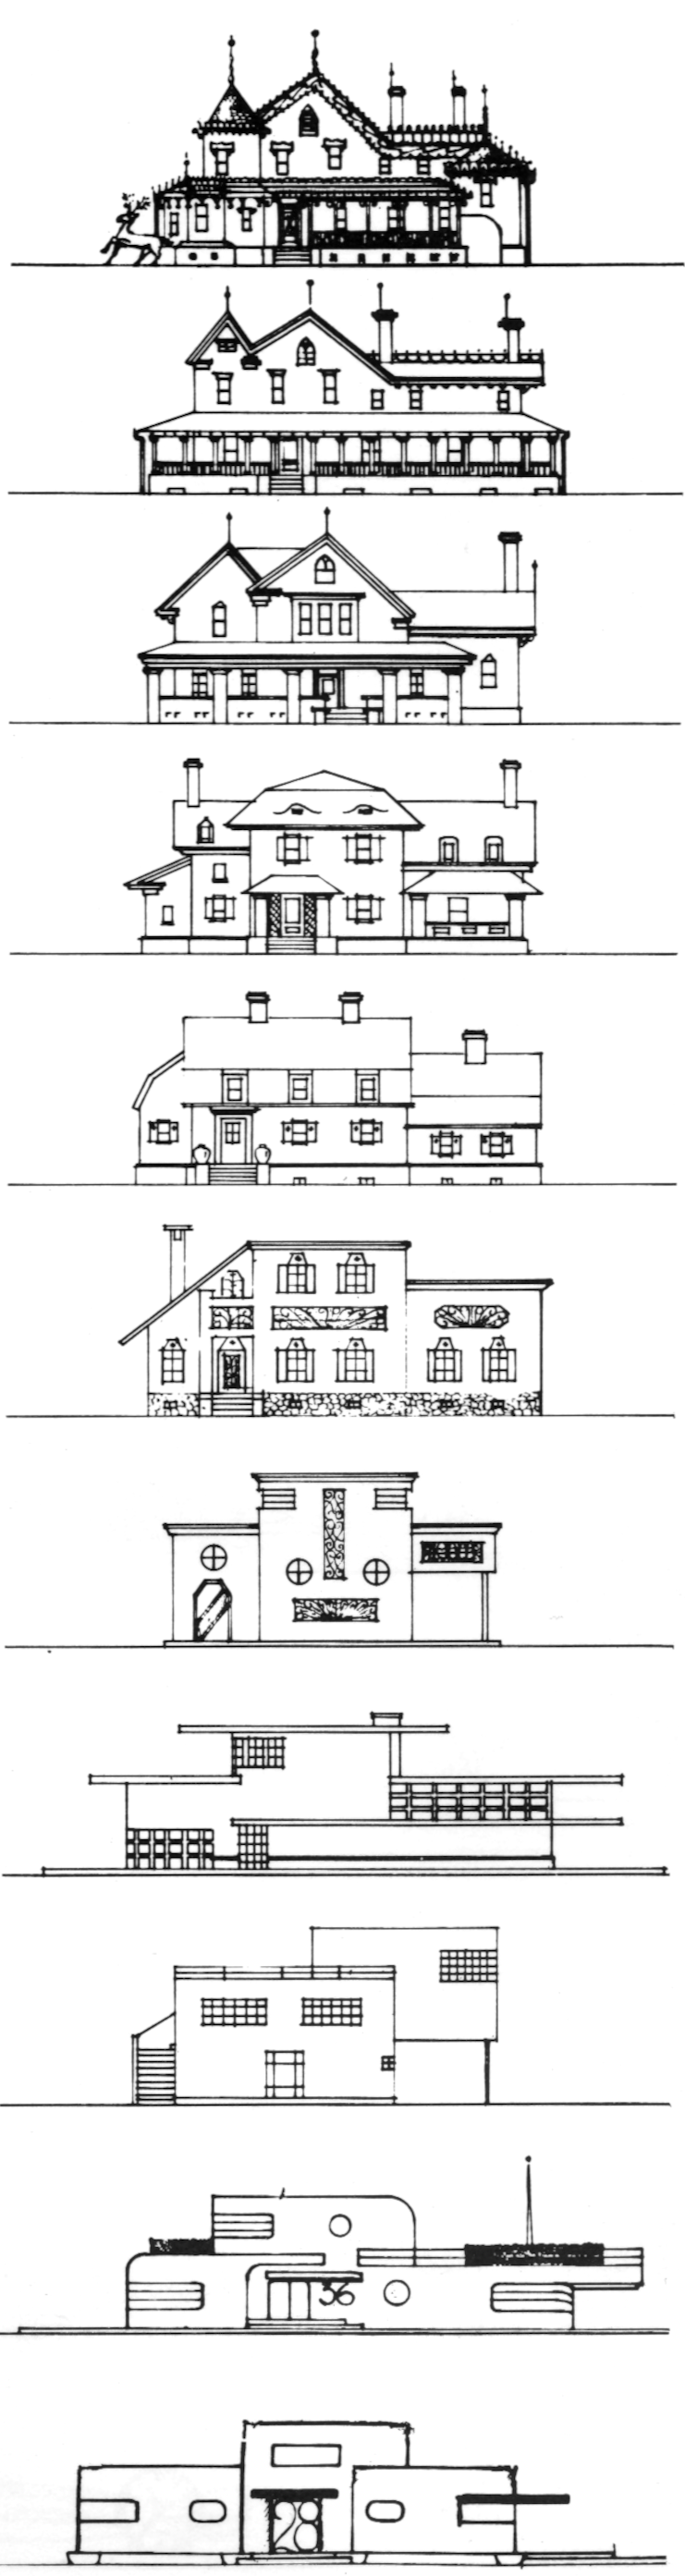
\includegraphics[width=50mm]{./figures/loewy_architecture.png}
    \caption{
        "Design Evolution 1930" by French-born American industrial designer Raymond Loewy \cite{loewy_industrial_1979}
    }
    \label{fig:loewy}
    \end{figure}
\end{minipage}

\clearpage
\section{The Age of Construction}

\begin{multicols}{2}

Recent data collected by the International Energy Agency shows that the construction of new buildings is expected to add a floor area equivalent to the surface of the city of Paris every week all the way through 2050 \cite[Sec. 3.7]{cozzi_net_2021}.

At the same time, the urban planning offices of several European countries expect and plan for an average service life of newly constructed buildings on the order of only 50 years. The exact lifetime depends on a number of factors, including the purpose of the structure (data for Denmark: 100 years for single-family homes, 75 years for cultural buildings and 50 years for health or teaching buildings \cite{andersen_lifespan_2023}). Further significant differences between the age of the building stock between different countries exist, with buildings in France having a significantly shorter lifetime \cite{noauthor_value_2013} than those in Switzerland \cite{kornmann_service_2012}.

An in-depth investigation of the underlying reasons for the short service life of the majority of the building stock remains an area of active research. In the context of this proposal, we will mention only two:

First, the changing demand structure in the context of residential buildings.

Ongoing societal transformations have driven a continuing trend towards fewer children per family and an increase of single-person households. This trend is illustrated in \cref{fig:households}. New construction of residential buildings is therefore seen as an opportunity to increase urban density by catering to smaller households, avoiding often equally expensive large-scale structural modifications of existing building stock. This trend is so significant that despite low birth rates in industrialized nations, the number of households has grown significantly, even without accounting for migration \cite{noauthor_why_2014}.

It should be noted that the degree of bi-directional causality between an increasing supply of smaller dwellings and family size at the advanced state of this trend has not been conclusively investigated \cite{kulu_fertility_2007}. For instance, the 2021 edition of the U.S. Census Bureau American Community Survey showed fertility rates for occupants of single-family homes to be significantly larger than occupants of apartment buildings \cite{noauthor_american_2021}. Decreasing the supply of larger dwellings on the housing market could induce a feedback loop, whereby the decreasing space of apartments decreases statistical fertility, necessitating even more new construction.

\end{multicols}

\begin{figure}[ht!]
    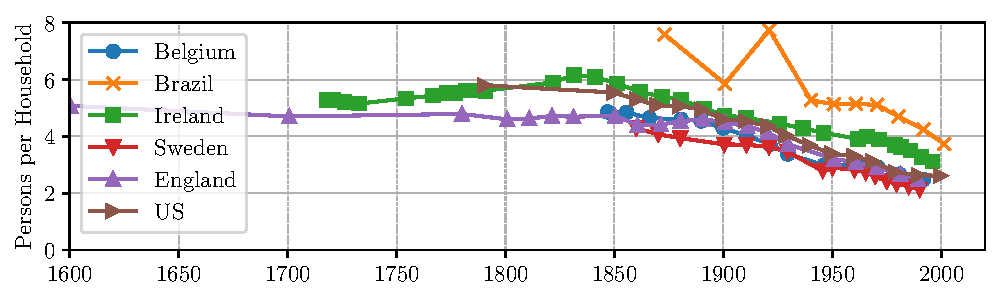
\includegraphics[width=\textwidth]{./figures/household_size.pdf}
    \vspace{-5mm}
    \caption{
        Average household size for different countries between 1600 and 2000. Each point represents average household size during the census for the corresponding year. The figure illustrated how the average number of people living in a household has been shrinking in developed countries for centuries, with the pace of this change accelerating in the early 1900s. A statistical analysis of the data by the authors of the original study shows 
        a significant change in the trend of household size for developed nations around the year 1893. The authors concluded: \textit{"the number of households grew faster than population size in every country and every time period."}. Figure source: Own rendering, with data adapted Mason et al. \cite[Figure 2]{bradbury_long-term_2014}
    }
    \label{fig:households}
\end{figure}

\clearpage
\begin{multicols}{2}

Second, the "diminishing climate returns" of extending building service-life.

The construction and maintenance of buildings in 2022 was responsible for 40\% of global carbon emissions \cite{camarasa_energy_2023}. Consequently, policy makers have been focusing on \textit{"accelerating and rapidly scaling up energy efficiency measures"} in the construction sector \cite{noauthor_2022_2022}. Researchers of the Intergovernmental Panel on Climate Change (IPCC) Working Group for Climate Change Mitigation in recently re-affirmed the emissions reduction potential that the sector offered. Proposed measures include improving existing buildings efficiency and use, high-performance new buildings, integrating renewable energy production in buildings, and decarbonizing production of building materials \cite{shukla_mitigation_2022}.

In this context, the energy expenditure and associated carbon emissions of the construction sector have recently come under increasing scrutiny from researchers in the field of industrial ecology, life-cycle assessment and sustainable construction \cite{chau_review_2015}\cite{ortiz_sustainability_2009}. A key finding is illustrated in \cref{fig:energy}: While extending the lifetime of buildings decreases the carbon emissions associated with its use, this effect naturally decreases over the lifetime of the building, as the recurrent carbon emissions from necessary refurbishment accumulate. Constructing an entirely new building to higher energy efficiency standards is therefore often seen as the preferable option for buildings over a certain age.

This, of course, is in contrast to World Green Building Council: \textit{"The most sustainable building is ironically, the one not built"}

\textit{"Reducing the use of high-volume, carbon-intensive materials such as concrete, steel and plastics, and replacing them with low-carbon and circular alternatives, should be the main approach."} \cite[Sec. 7.4]{noauthor_2022_2022}

Ultimately, many proposed to decarbonize the economy are challenging for technical and political reasons. This includes a reduction of personal mobility, additional taxes on flights or the electrification of sectors with \textit{hard to abate} carbon emissions. At the same time, some of the most straightforward pathways remain unexplored - for instance: \textit{"Don't design houses for a 50 year service life."}.

\end{multicols}

\begin{figure}[ht!]
    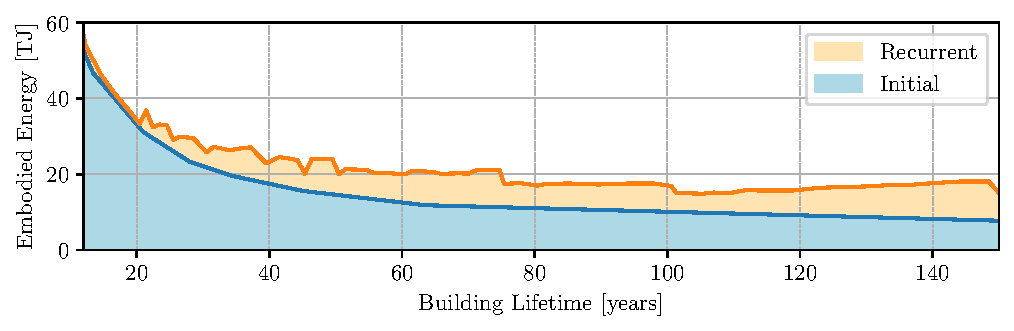
\includegraphics[width=\textwidth]{./figures/building_embodied_energy.pdf}
    \vspace{-5mm}
    \caption{
        Life-cycle embodied energy of a single-storey detached house by building service life. The functional unit of the assessment is the provisioning of the case-study building over a period of 150 years. A building lifetime of 15 years assumes that the house is torn down and rebuilt 10 times during the 150 year investigated timeframe. In this case, the figure show that the majority of energy is expended on the reconstruction ("initial"). On the other hand, a building lifetime of 150 years assumes that house is never torn down in the investigated timeframe. In this case, the figure shows that the majority of the energy is expended on refurbishment and renovation ("recurrent").
        \newline Figure source: Own rendering, with data adapted from Rauf and Crawford \cite[Figure 5]{rauf_building_2015}
    }
    \label{fig:energy}
\end{figure}

\clearpage
\section{Aesthetics}
\label{sec:aesthetics}

Modern architecture is always ugly. Nonetheless, we limit our discussion to buildings of a representative nature. We exclude housing (eg. apartment complexes) to avoid:

As we have seen illustrated in the proclamations of Corbusier and XXX, "Taste is subjective" (and we must take part in) has always been the the refuge of modernists. Corbusier said that the public had to be re-educated, and others have wondered about the vulgarity of designs for the public and asked whether architects should take these architectural tastes seriously.

\clearpage
\section{Democracy}

\begin{multicols}{2}

While the role of art in a free society remains a topic of philosophical debate, contemporary scholars agree that the role of art in democracy can be non-exhaustively defined as a mode of participation and action that engages the public in dialogue and debate, and that inspires social change and transformation. Art thereby can be seen not only as the highest form of self-expression but also as a vital element of the democratic process.

Architecture, unlike some of the fine arts, generally serves an immediate purpose beyond that of aesthetic or intellectual expression. In this way it can perhaps most graciously be described as adding to- and expanding on the functionality which civil engineers involved in any construction project aim to provide. This makes the designs of architects so ubiquitous in everyday life, that they been described as serving the function of \textit{a third skin}, on top of the anatomical and textile skins worn by man by Austrian artist and architect Friedrich Stowasser. As a result of its omnipresence in public space, it has been recognized as being

\textit{"(...) the most overweening of the arts, and the one that least lets us alone. A gallery we can't walk out of, a book we can't close, an art we can't even turn our back on because it is there facing us on the other side of the street as well (...)} - British poet Blake Morrison in "Lords of Glass, Steel and Concrete" \cite{morrison_lords_1982}

Switzerland is consistently ranked as of the most democratic nations globally \cite{noauthor_economist_2023} with the principles of subsidiarity and direct democracy forming a vital part of Swiss national identity. At the same time, home ownership remains elusive for the majority of the population, having stagnated at around 40\% over the past years \cite{noauthor_home_2022}. 

What does it say about the relationship between art and architecture and the public if 


How can citizens ensure that XXXX

\cref{sec:aesthetics}


\cref{fig:vienna} and \cref{fig:budaptest} show two diametrically opposed approaches to the replacement of existing building stock in cities that share a similar socio-economic and architectural legacy. 


Architects have been publicly calling for the public to be re-educated to appreciate their brutalist/modernist designs. (eg. the architects that build the Triemli Tower).

In fact, we can observe that there is a kind of self-propagating effect: architectural prizes are given out only by architects. There is no 'public vote'. The contempt with which architects have treated the public is by no means covert. This is perhaps best exemplified by the reaction of Rudolf Guyer, who in 1955 designed a high-rise residential apartment in souther Zurich. When the building was voted "Switzerland's ugiest building" in 2018 by readers of the daily newspaper \textit{20 Minuten}, he declared:

\textit{"Dass Laien das Gebäude hässlich finden, ist mir egal. Hauptsache, den anderen Architekten gefällt es."} (en.: I don't care that laypeople find the building ugly. The main thing is that the other architects like it) 


\end{multicols}

\begin{figure}[ht!]
    \centering
    \subfloat{{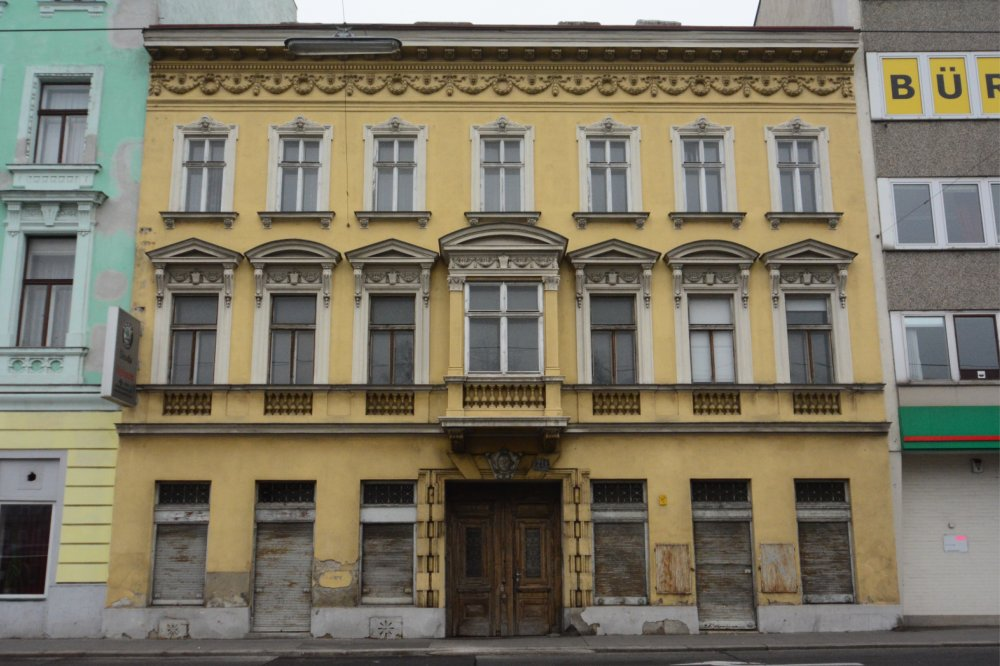
\includegraphics[height=5cm]{figures/vienna_1.jpg} }}
    \subfloat{{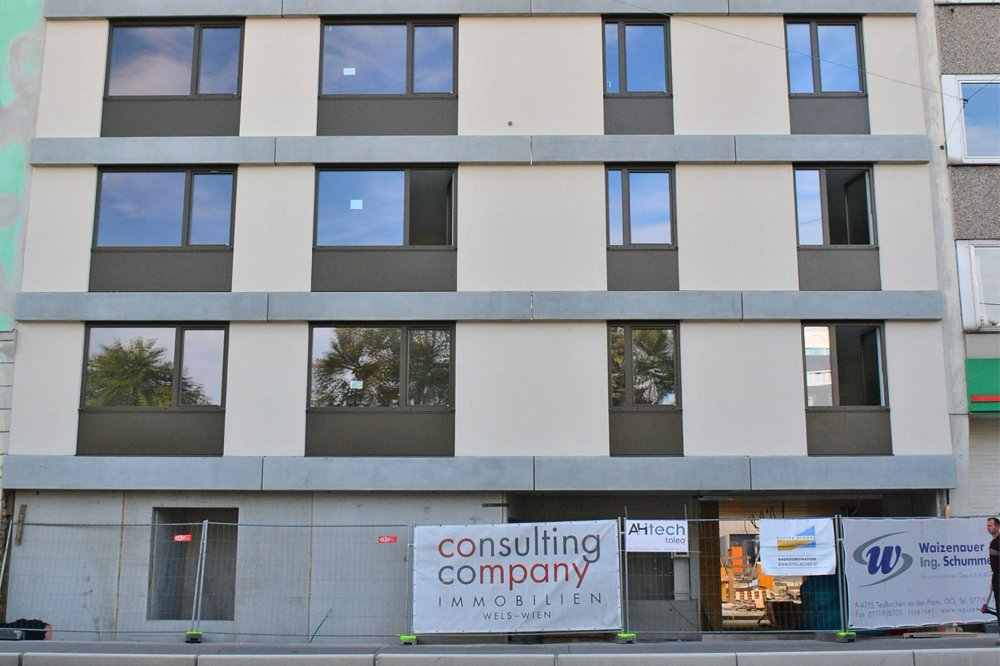
\includegraphics[height=5cm]{figures/vienna_2.jpg} }}
    \caption{Before-and-after: Demolition and reconstruction of a 19th century Gründerzeit style Vienna town house on Schönbrunner Strasse (12th District), as documented by Georg Scherer of the architecture watchblog \texttt{wienschauen.at} \cite{scherer_zerstorung_nodate}. Image sources (left to right): \cite{scherer_schonbrunner_2018}\cite{wikimedia_commons_user_guentherz_wohnhaus_2014}}
    \label{fig:vienna}
\end{figure}

\begin{figure}[ht!]
    \centering
    \subfloat{{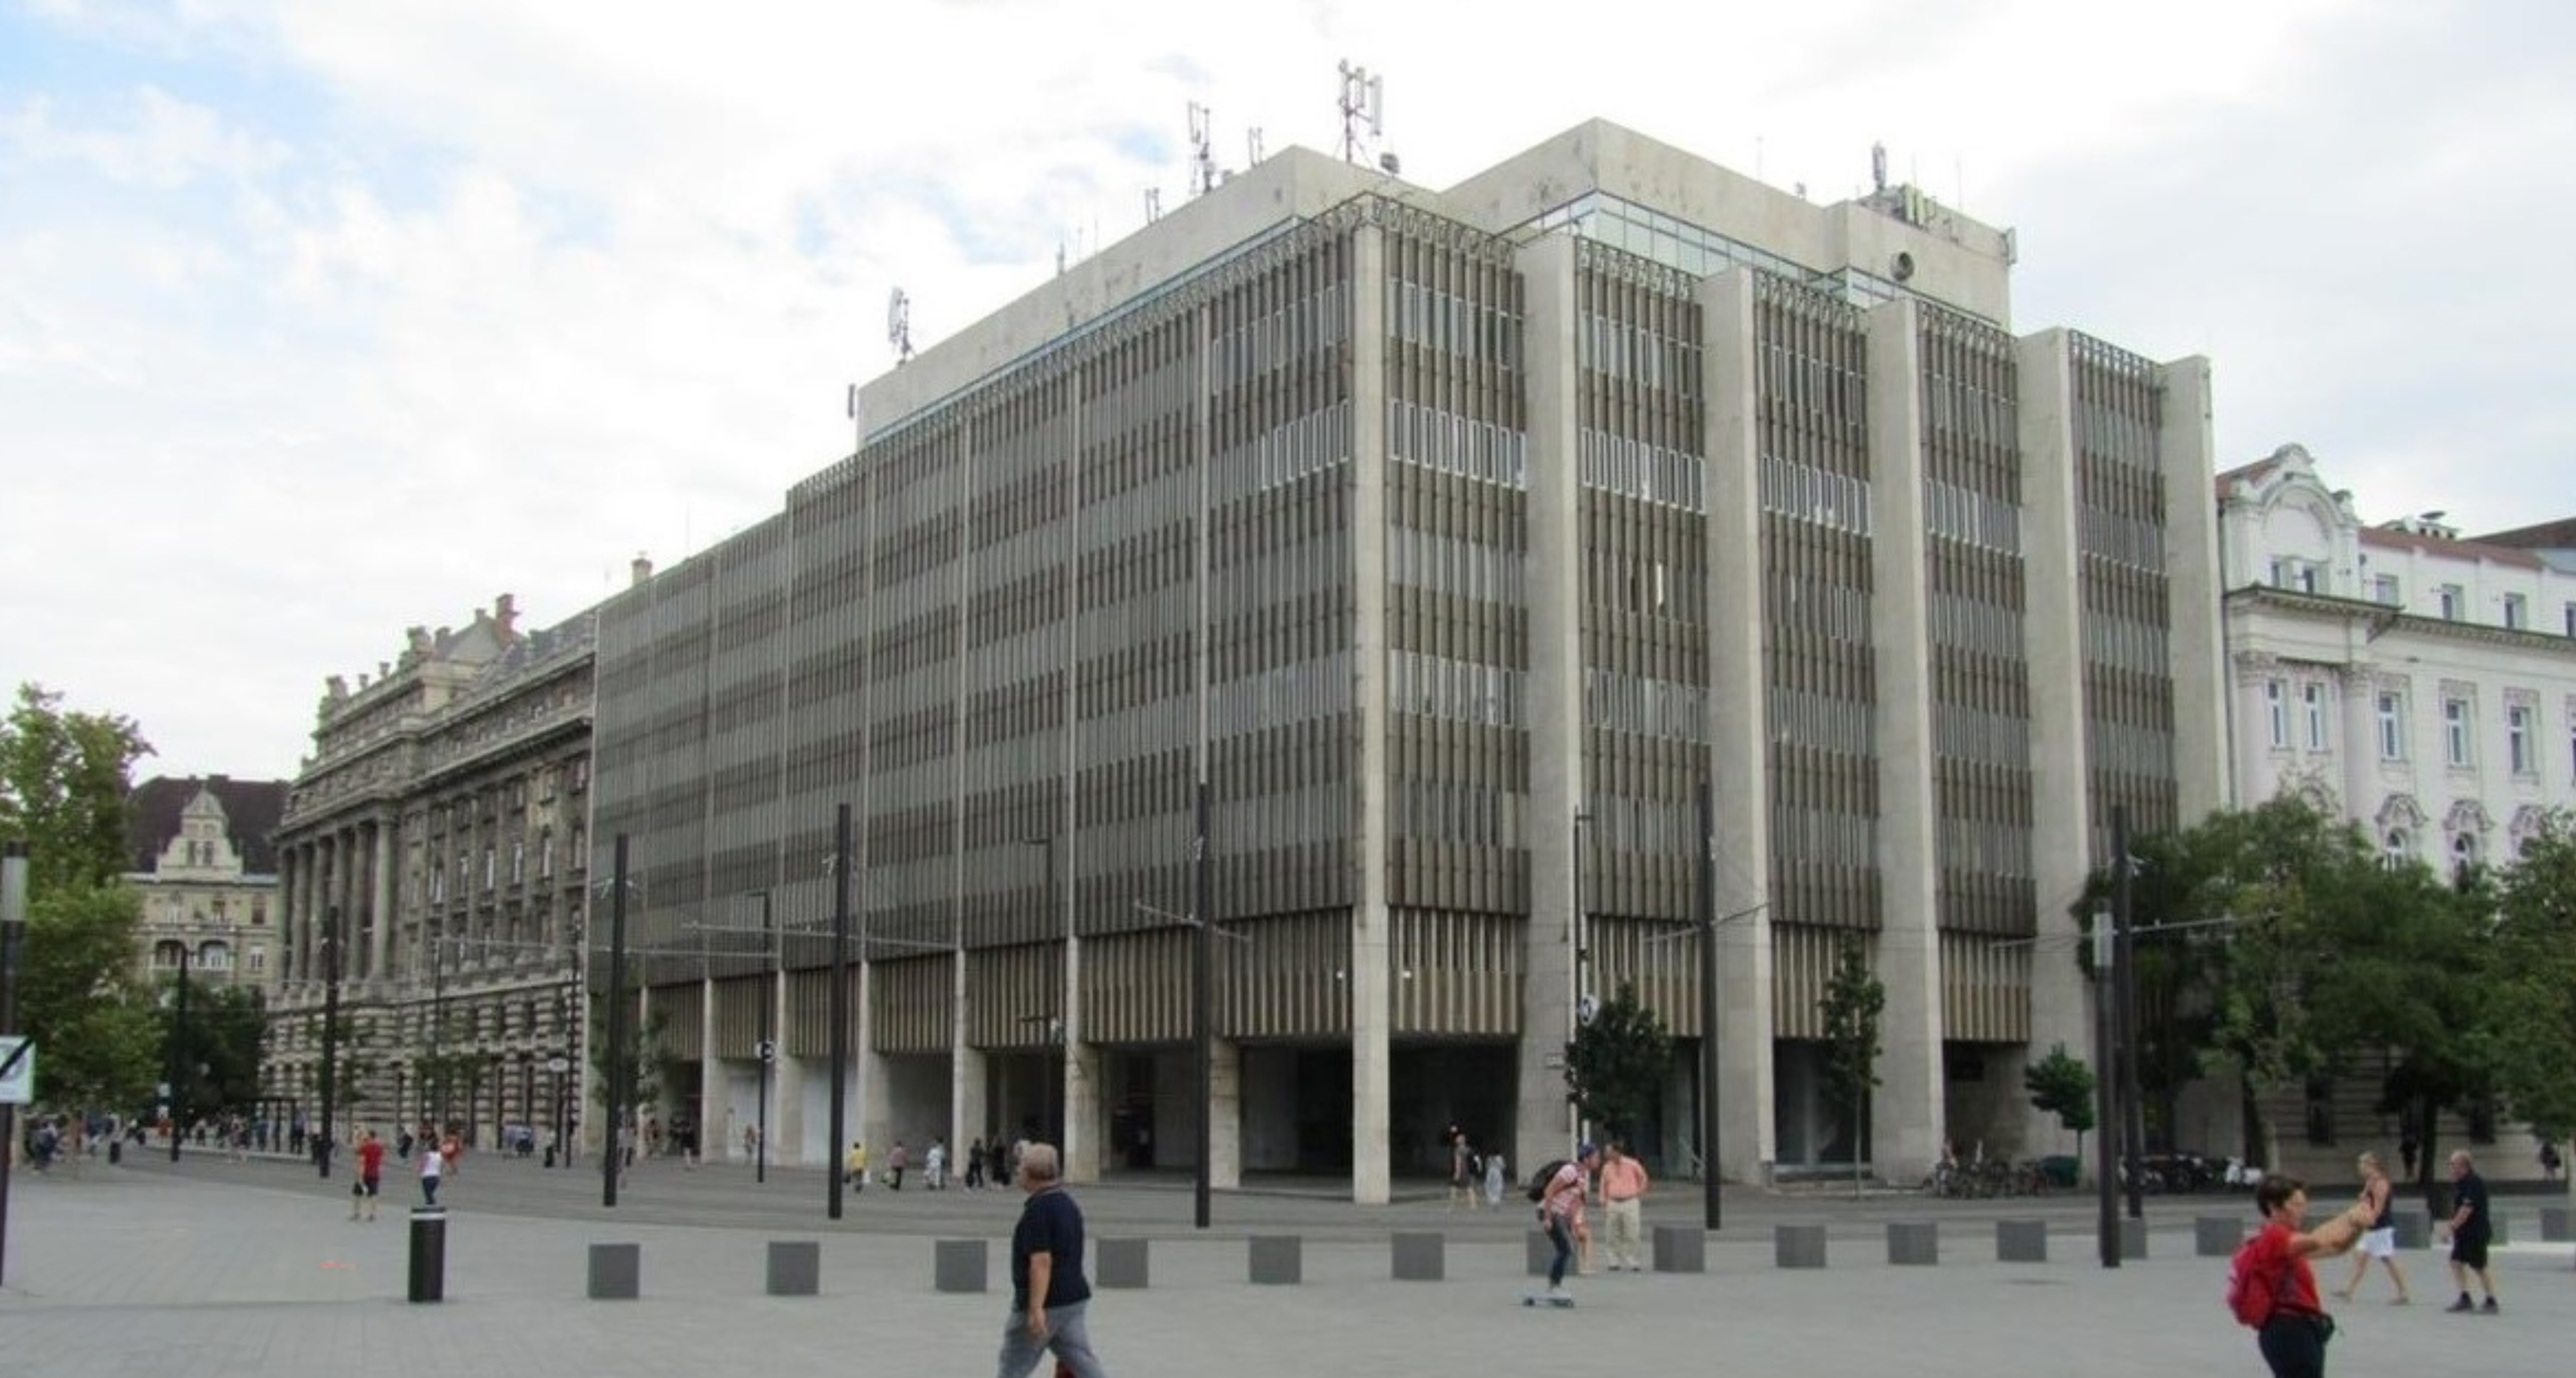
\includegraphics[height=4cm]{figures/hungary_1.jpg} }}
    \subfloat{{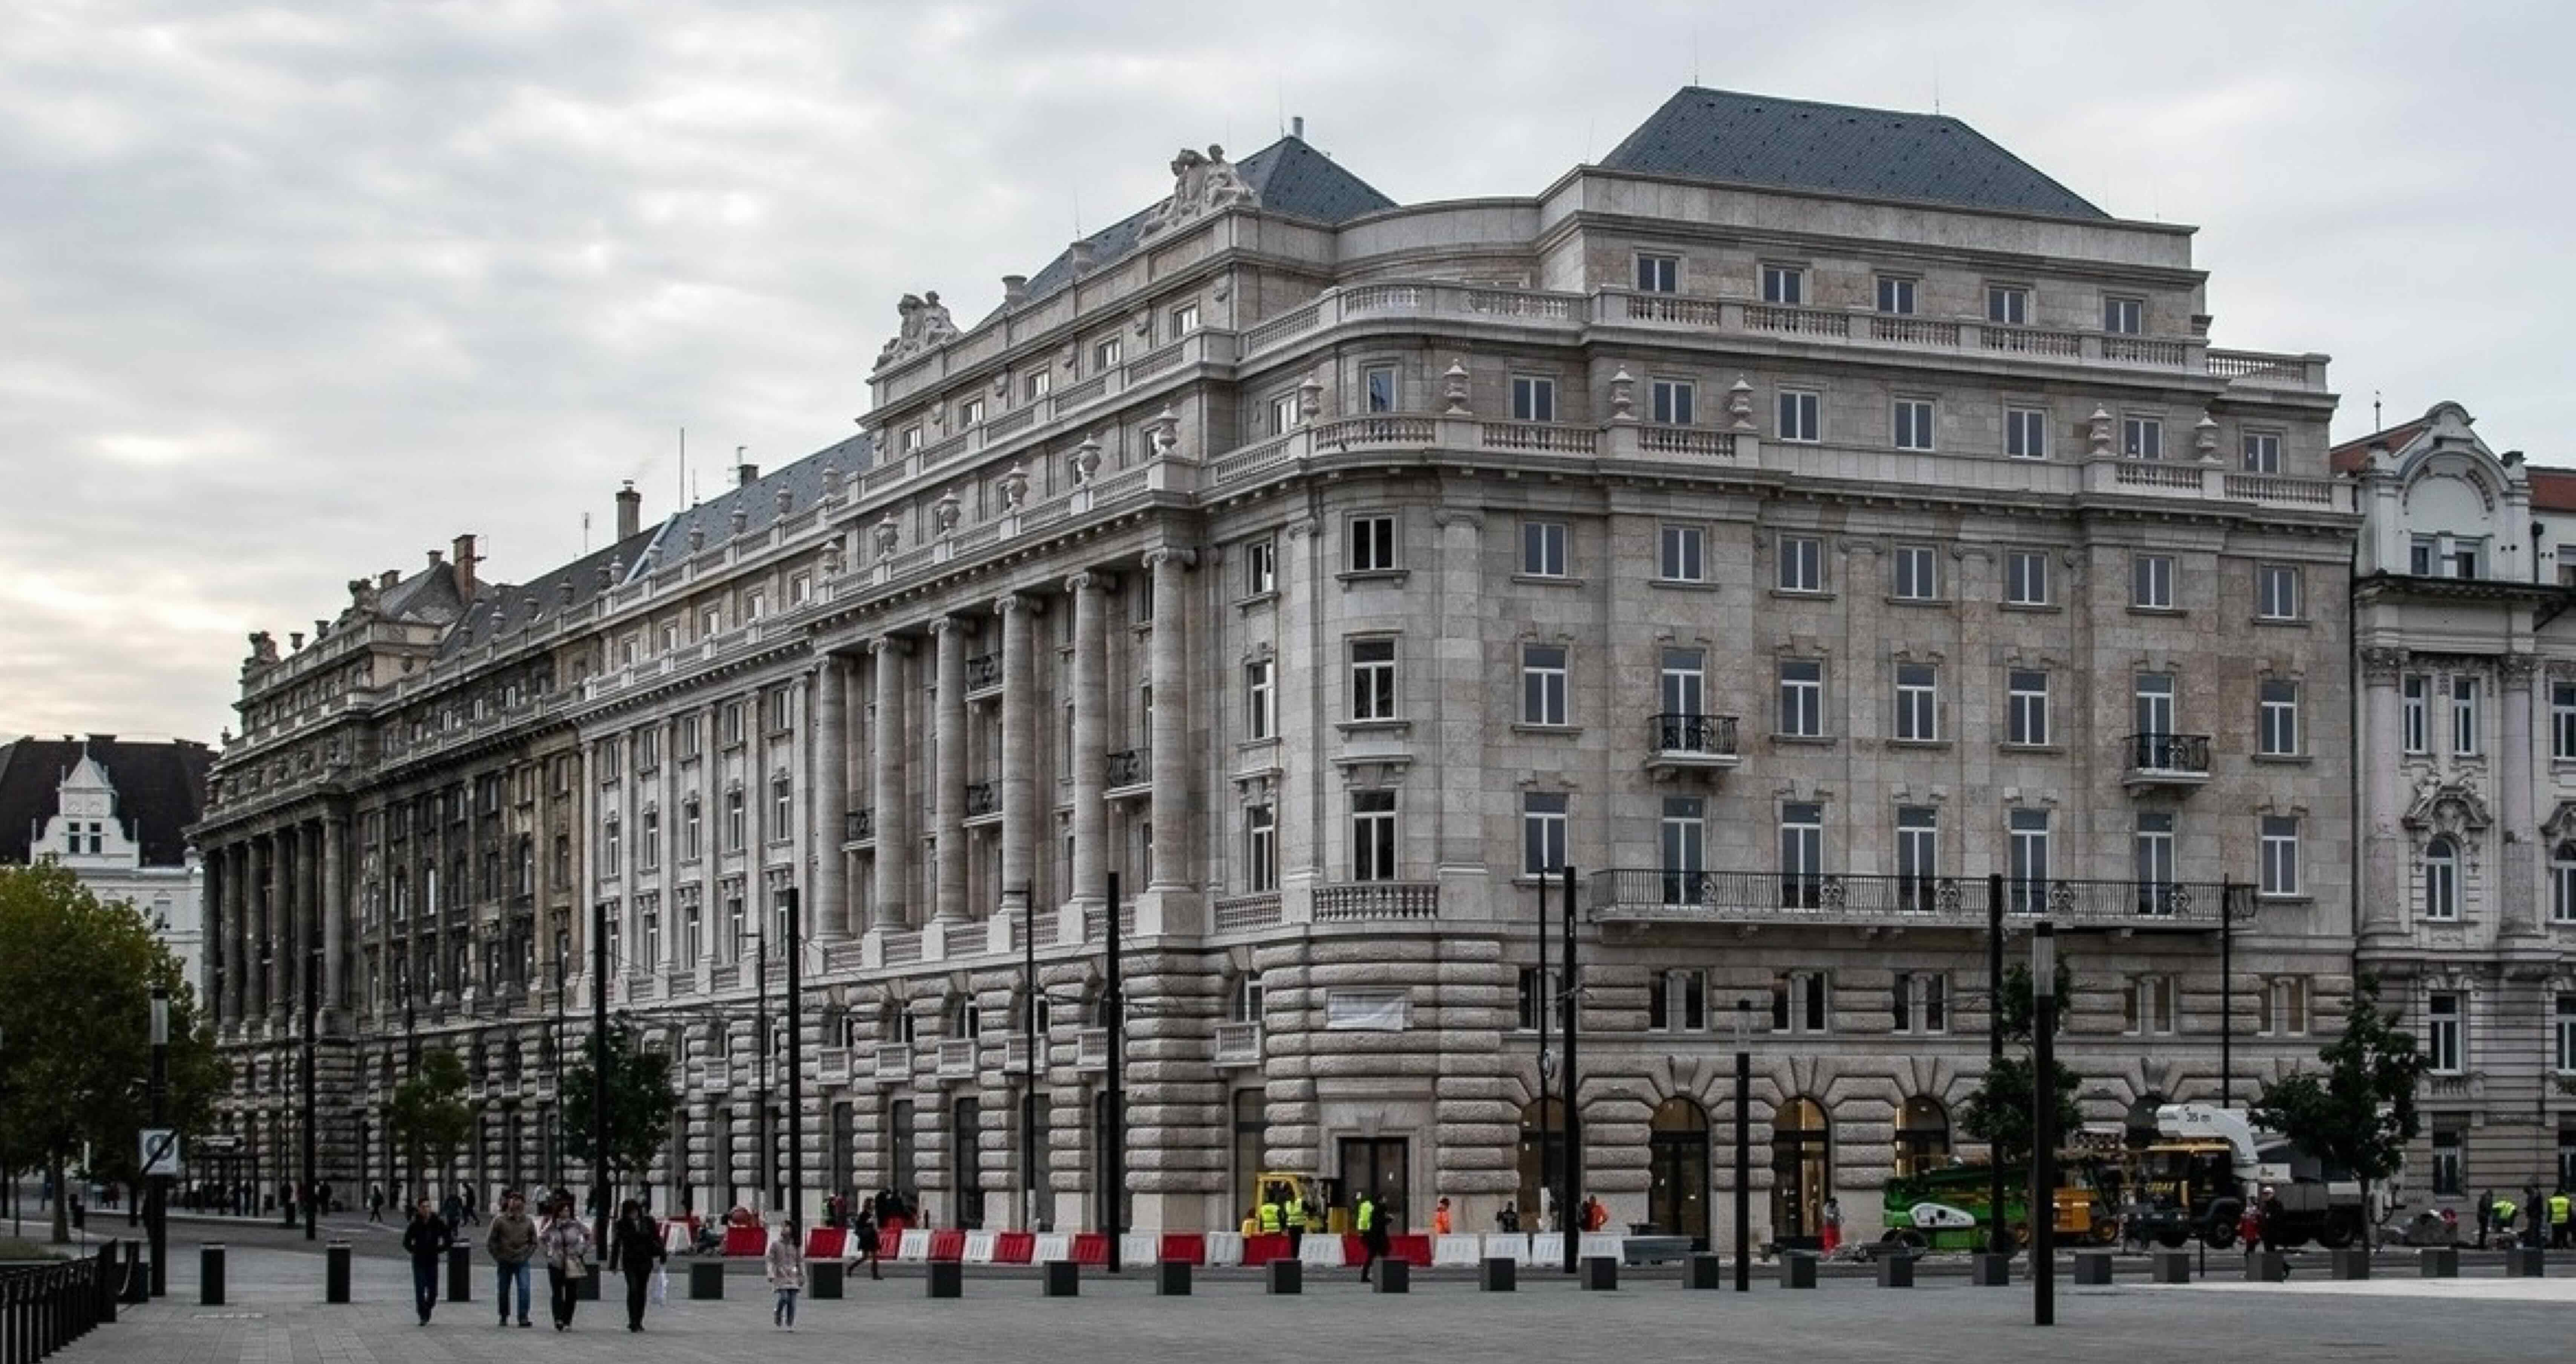
\includegraphics[height=4cm]{figures/hungary_2.jpg} }}
    \caption{Before-and-after: Demolition and reconstruction of a 1970s office building on Kossuth Lajos Square in Budapest, adjacent to the Hungarian Parliament Building, as documented by Michael Diamant of the architecture watchblog \texttt{newtrad.org}. The brutalist style design was intended to replace the unrealized wing of an earlier neo-classical style building. This wing was finally realized according to the original design following the demolition of the 1970s building. Image sources: Adapted from original photographs by Michael Diamant in \cite{natalia_michael_2021} }
    \label{fig:budaptest}
\end{figure}

\begin{figure}[ht!]
    \centering
    \subfloat{{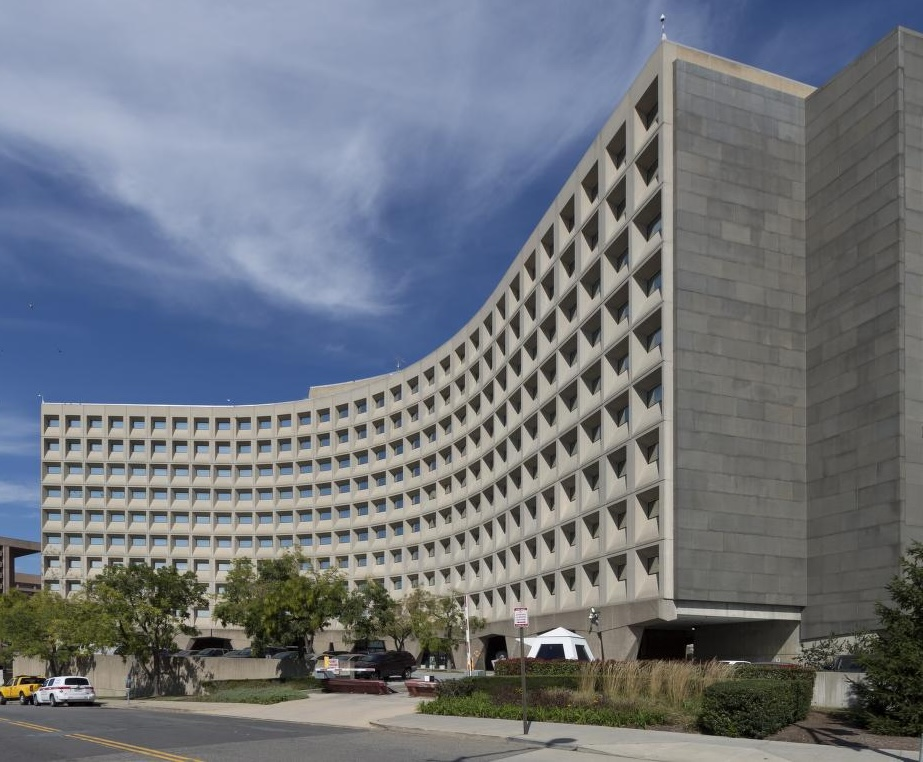
\includegraphics[height=5cm]{figures/us_gov_modernist_1.jpg} }}
    \subfloat{{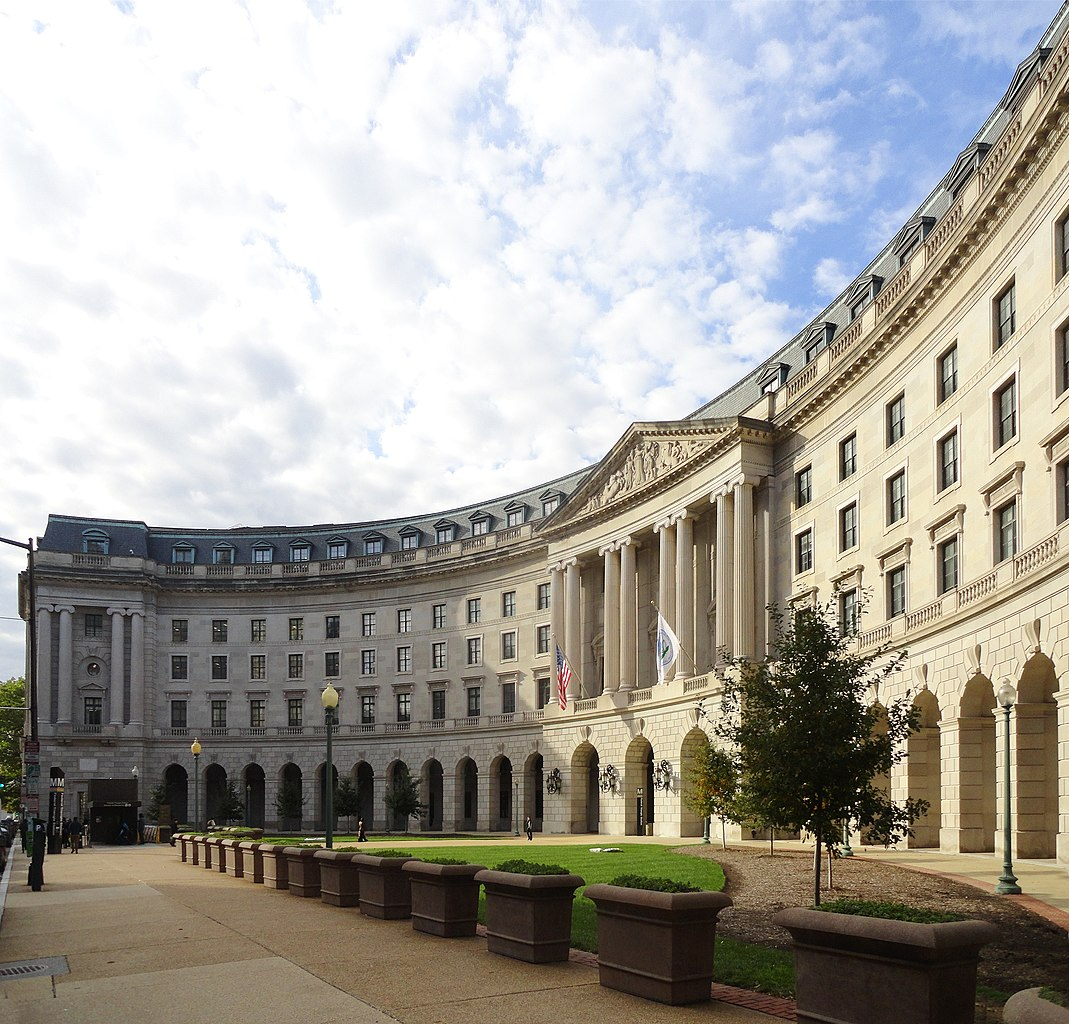
\includegraphics[height=5cm]{figures/us_gov_traditional_1.jpg} }}
    \caption{Left: The Robert C. Weaver Federal Building on 7th Street SW in Washington, D.C., designed in 1965 by Marcel Breuer. It presently serves as the headquarter of the United States Department of Housing and Urban Development. Note that the current occupancy of the building evokes Winston Churchill's famous quote: \textit{"We shape our buildings, thereafter they shape us."} \cite{noauthor_churchill_nodate}. Right: The William Jefferson Clinton Federal Building on Pennsylvania Avenue in Washington, D.C., designed in 1934 by William Adams Delano and Chester Holmes Aldrich. It presently serves as the headquarters of the Environmental Protection Agency. Images of this nature formed the core part of the 2020 American poll on architectural preferences \cite{noauthor_americans_2020}. All image pairs presented showed images of similar shape and purpose, thereby accounting for major non-aesthetic considerations. \newline Image sources (left to right): \cite{highsmith_robert_2012}\cite{wikimedia_commons_user_moreau1_epa_2018}}
    \label{fig:federal_buildings}
\end{figure}

\begin{figure}[ht!]
    \centering
    \subfloat{{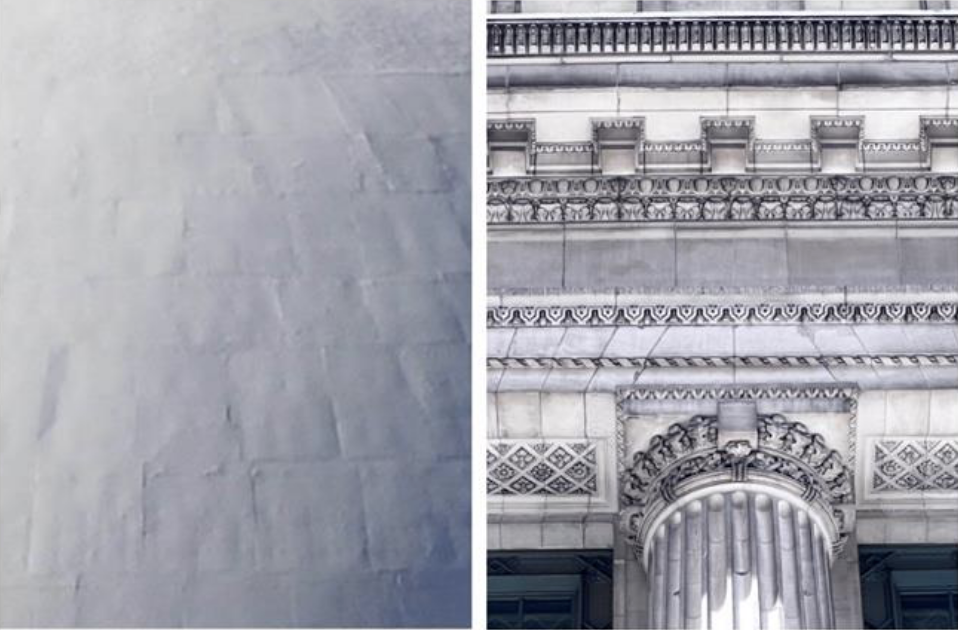
\includegraphics[height=5cm]{figures/beautyscale_image.png} }}
    \subfloat{{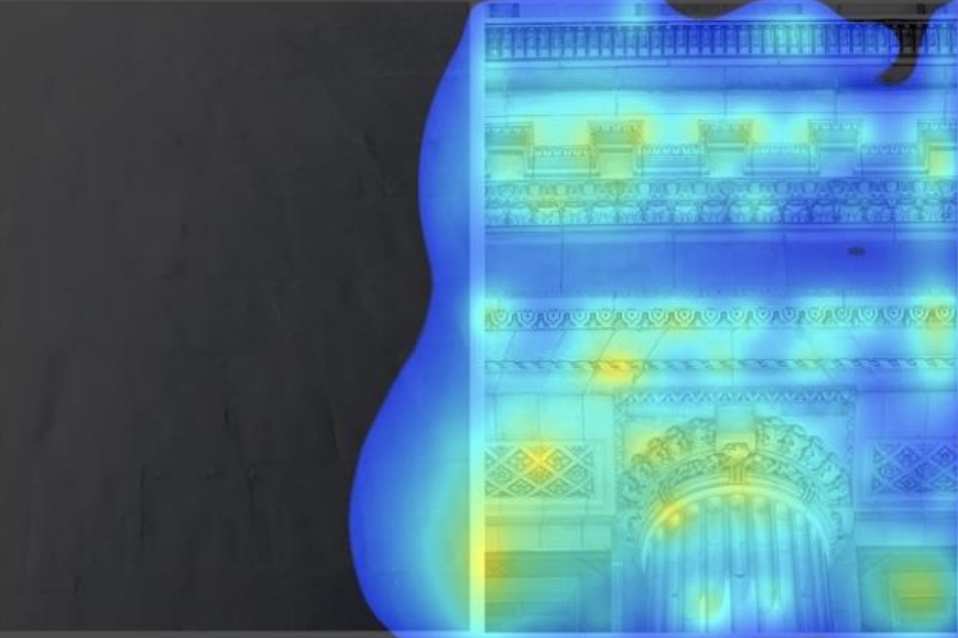
\includegraphics[height=5cm]{figures/beautyscale_heatmap.png} }}
    \caption{Left: Two designs for a building facade. Right: A heatmap reveals the degree to which the two different facade designs capture the attention of study participants. The heatmap was generated from eye-tracking data. As expected, the feature-rich pillar capital and lower-side cornice of the right facade retains visual attention to a much higher degree. Source:Figure 6 from Lavdas' and Salingaros' seminal publication \textit{"Architectural Beauty: Developing a Measurable and Objective Scale"} \cite{lavdas_architectural_2022}}
    \label{fig:heatmap}
\end{figure}

\begin{figure}[ht!]
    \centering
    \subfloat{{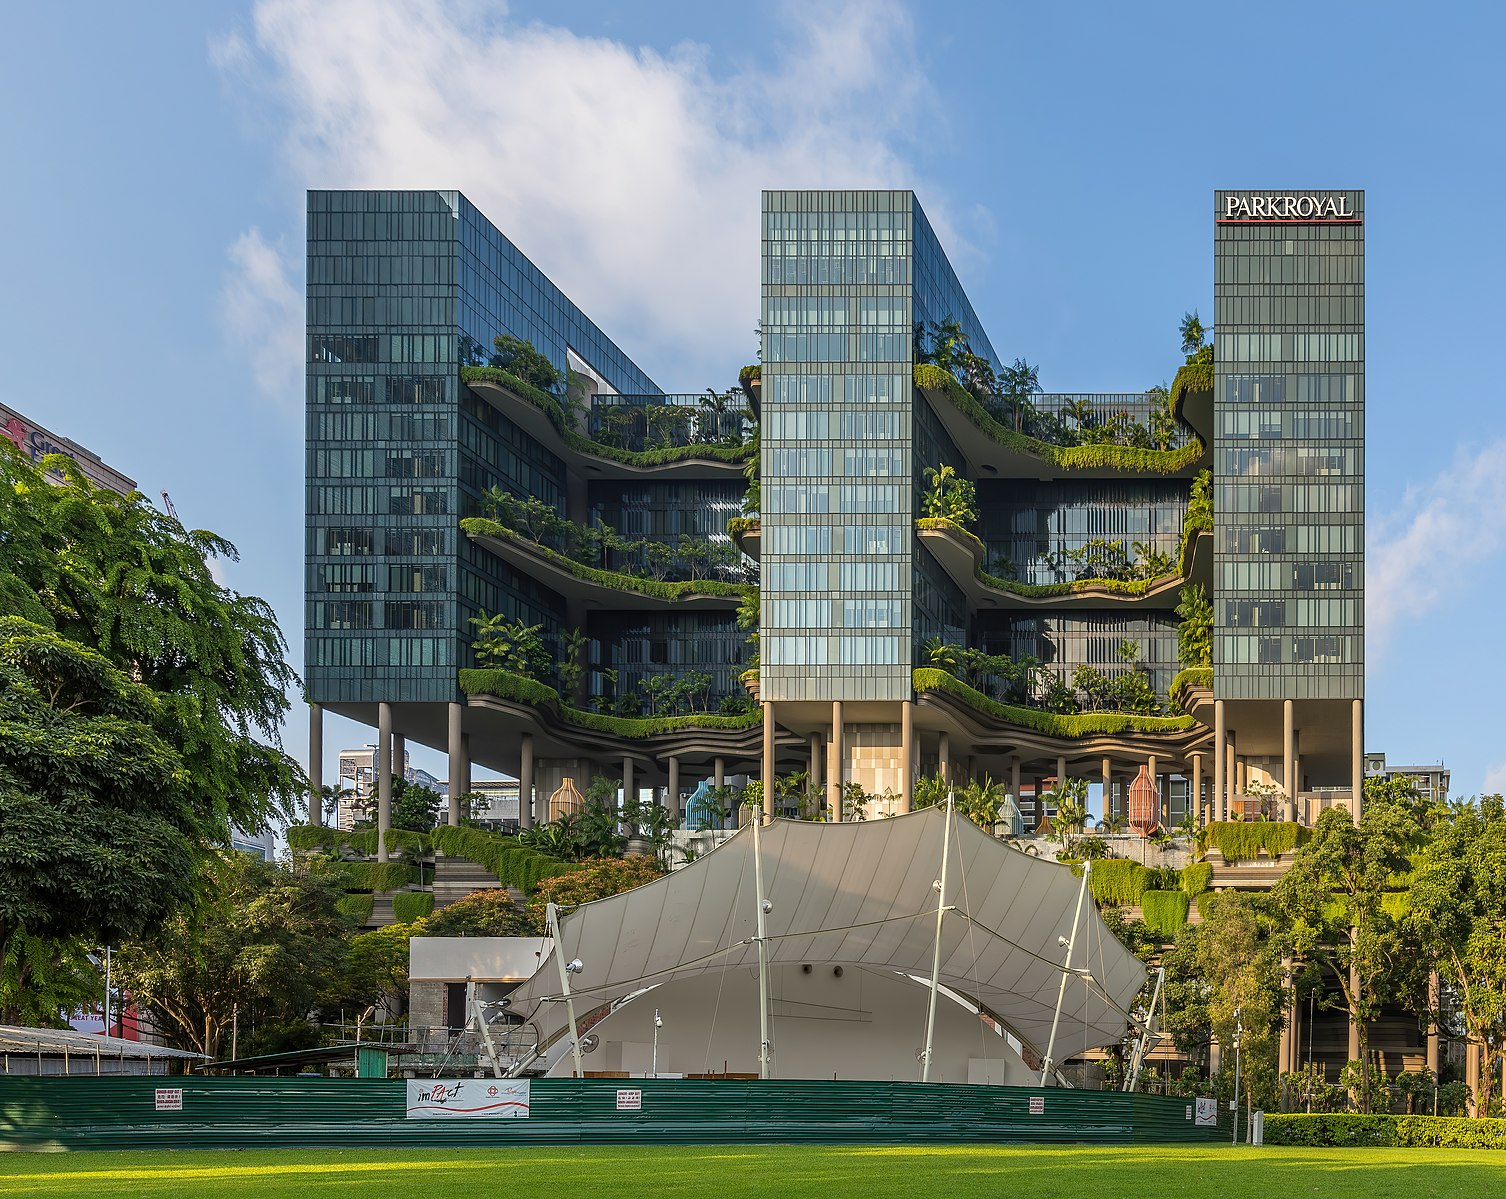
\includegraphics[height=5cm]{figures/parkroyal_1.jpg} }}
    \subfloat{{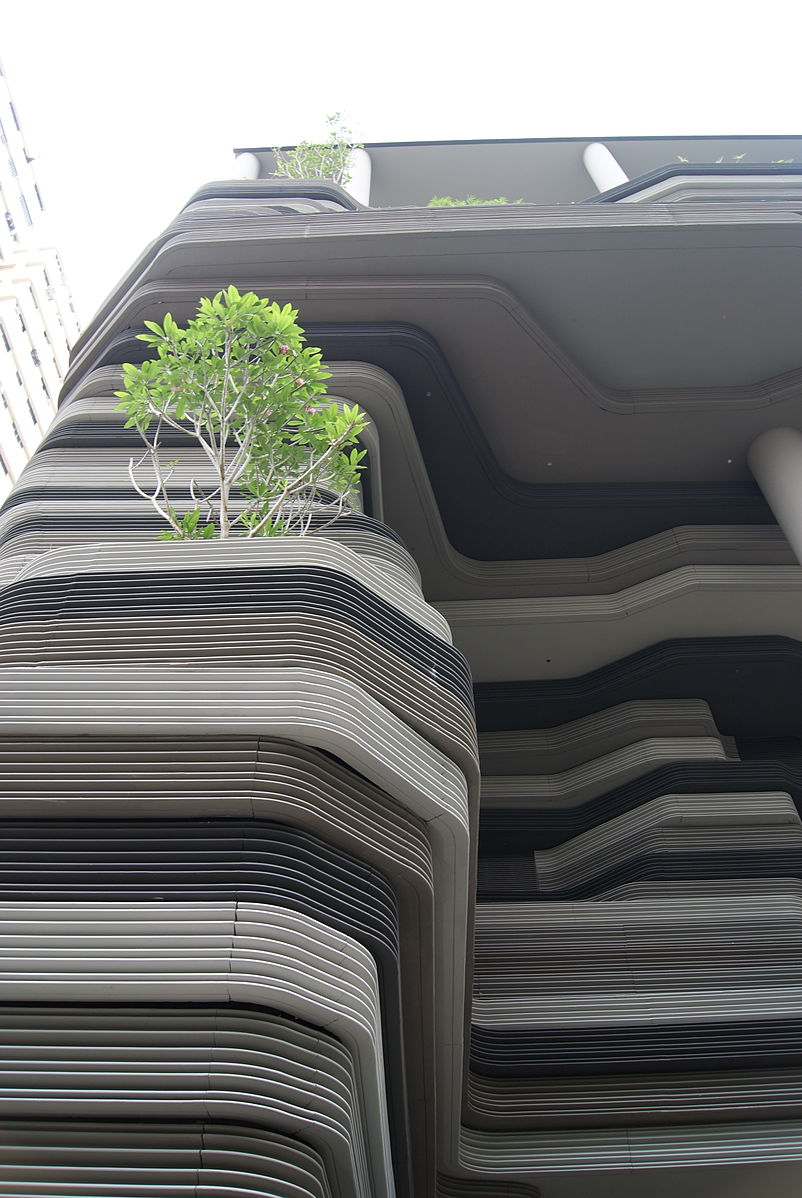
\includegraphics[height=5cm]{figures/parkroyal_2.jpg} }}
    \caption{The \textit{Parkroyal Collection Pickering} luxury hotel on Upper Pickering Street in Singapore, designed by members of the firm WOHA in 2013. Often described as a "garden in a hotel" \cite{hill_take_2021}, the building features multiple terrace gardens utilizing rainwater collection as part of its water management system. Left: Frontal view of the hotel from Hong Lim Park. Right: Detail of the concrete facade with solitary vegetation. \newline Image sources (left to right): \cite{morin_hotel_2018}\cite{smu_constitutional_and_administrative_law_wikipedia_project_parkroyal_2013}}
    \label{fig:parkroyal}
\end{figure}

\clearpage
\section{Biophilic Design}

\subsection{Biophilic Design for Aesthetics}

\begin{figure}[ht!]
    \centering
    \subfloat{{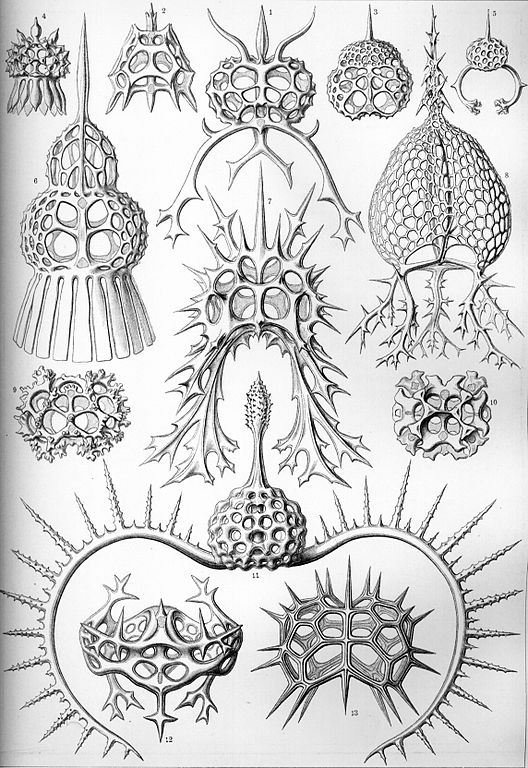
\includegraphics[height=5.5cm]{figures/Spyroidea.jpg} }}
    \subfloat{{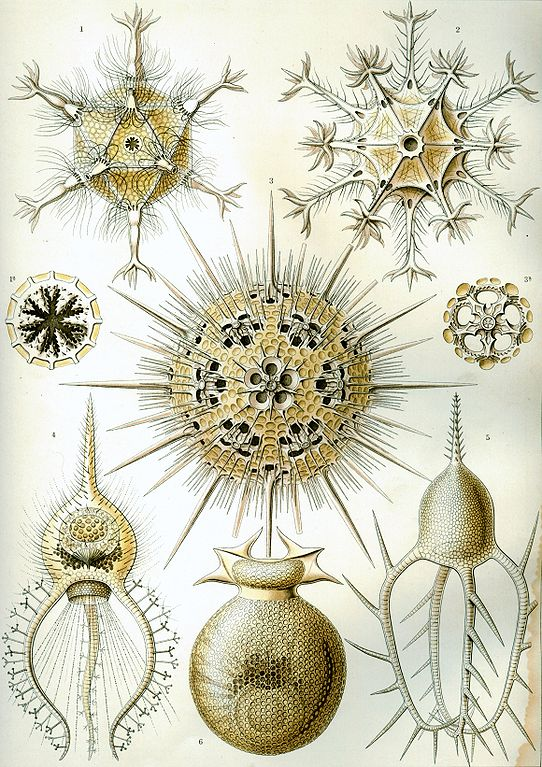
\includegraphics[height=5.5cm]{figures/Phaeodaria.jpg} }}
    \subfloat{{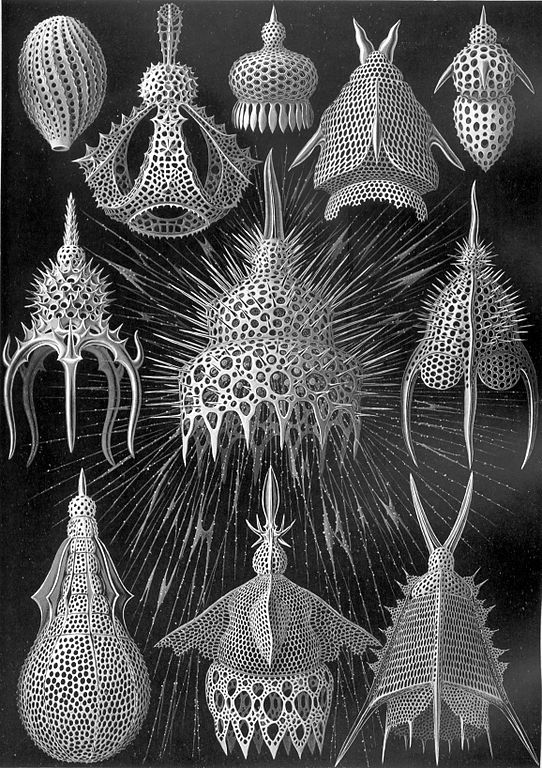
\includegraphics[height=5.5cm]{figures/Cyrtoidea.jpg} }}
    \caption{Selection of drawings from Ernst Haeckel's \textit{Kunstformen der Natur} (en.: "Art Forms in Nature") \cite{haeckel_kunstformen_2012}. According to architect Rene Binet, these drawings served as direct inspiration for his monumental arch \cite[Sec. "Haeckel und der Jugendstil"]{willmann_haeckel_2019}, which is depicted in \cref{fig:porte_binet}. \newline Image sources (left to right): Spyroidea \cite{haeckel_kunstformen_1904}, Phaeodaria \cite{haeckel_kunstformen_1904} and Cyrtoidea \cite{haeckel_kunstformen_1904-2}.}
    \label{fig:kunstformen}
\end{figure}

\begin{figure}[ht!]
    \centering
    \subfloat{{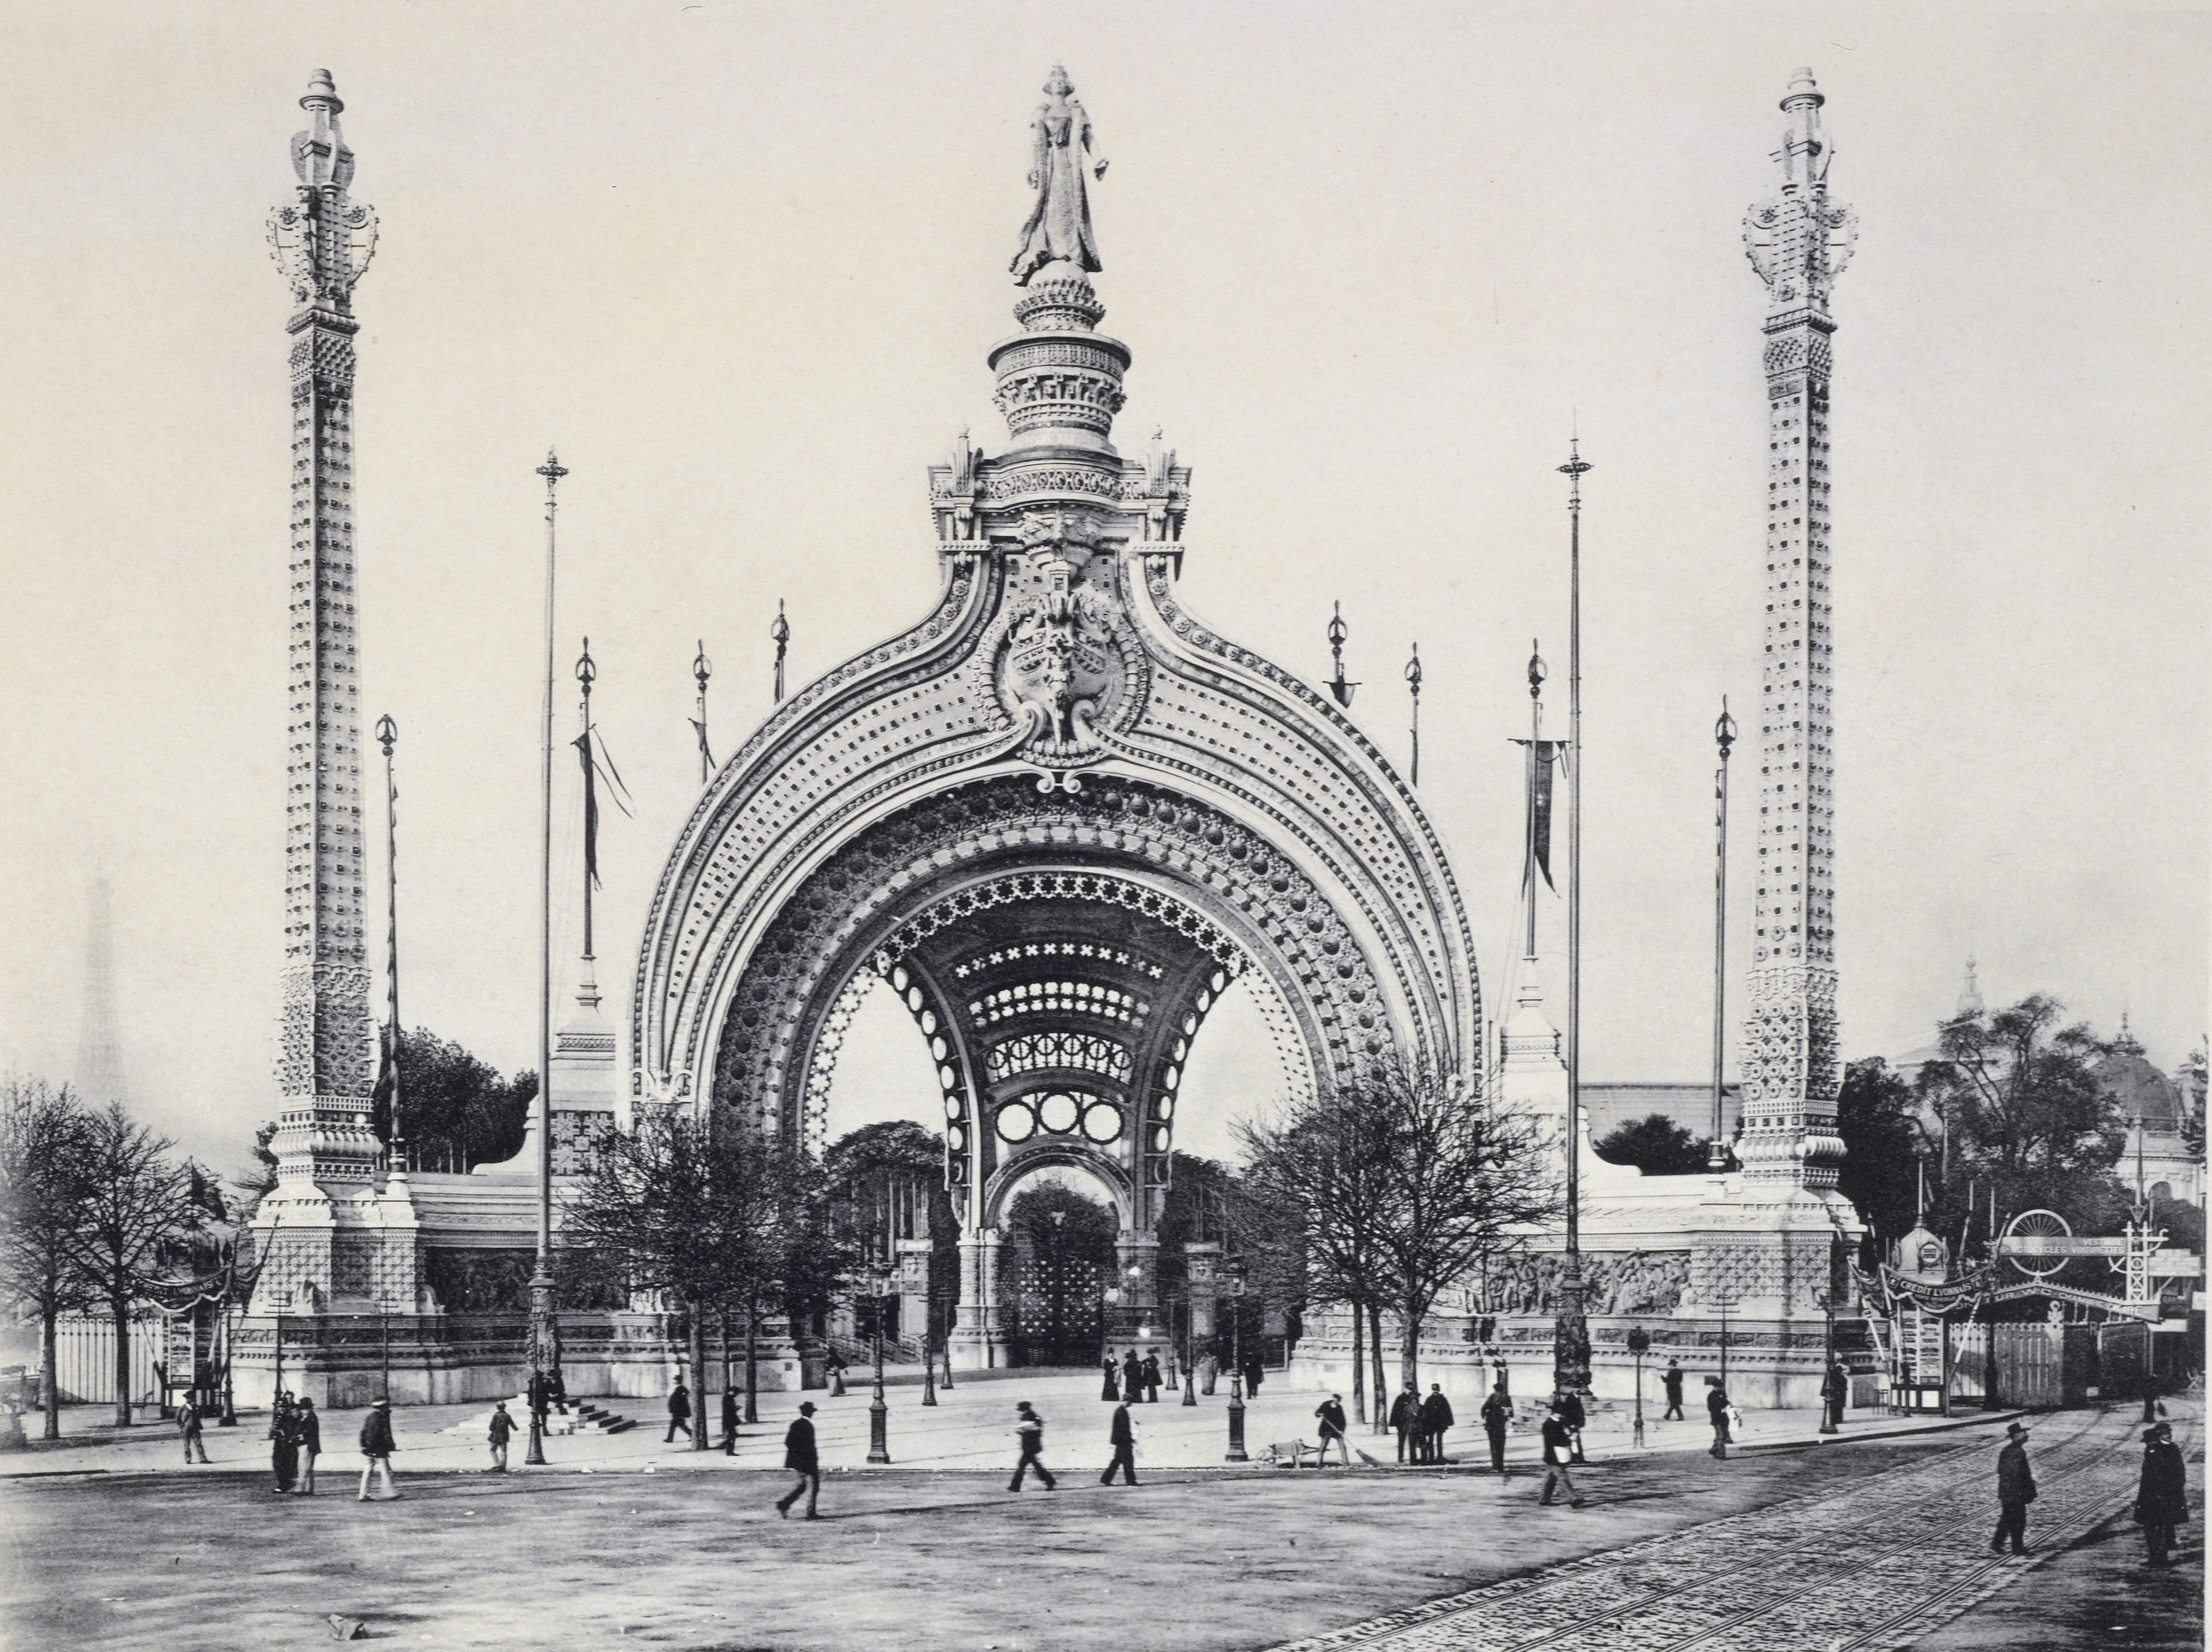
\includegraphics[height=5cm]{figures/porte_photograph.jpg} }}
    \subfloat{{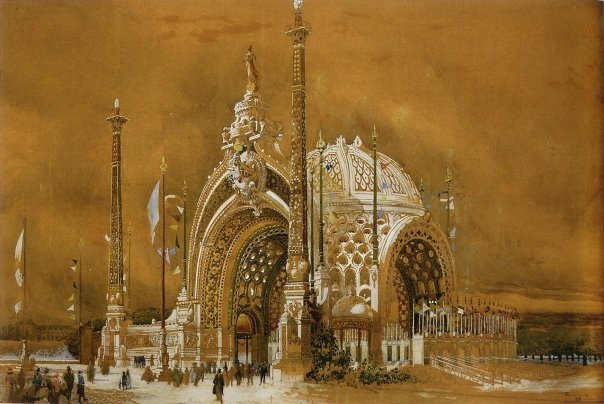
\includegraphics[height=5cm]{figures/porte_watercolor.jpg} }}
    \caption{Two renderings of the \textit{Porte Binet}, a monumental entrance at the site of the 1900 Paris Exhibition, designed by Rene Binet. The structure was composed of a metallic network with embedded coloured glass elements covering over 3000 electric lamps. \newline Image sources (left to right): \cite{louis_porte_1900}, \cite{binet_projet_1898}.}
    \label{fig:porte_binet}
\end{figure}

\clearpage
\subsection{Biophilic Design for Function}

\begin{figure}[ht!]
    \centering
    \subfloat{{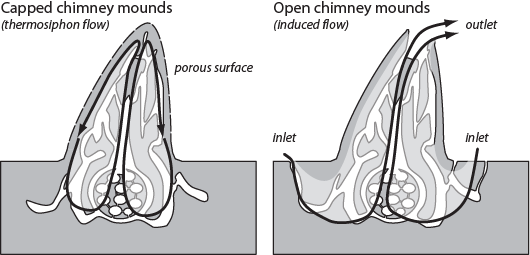
\includegraphics[height=4cm]{figures/termite_crossection.png} }}
    \subfloat{{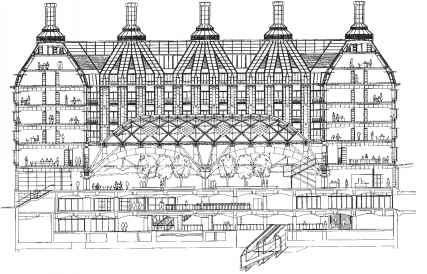
\includegraphics[height=5cm]{figures/portcullis_crossection.jpg} }}
    \caption{Perhaps the most famous example of functional bio-mimicry in the built environment: Energy-efficient air-flow cooling inspired by the design of termite mounds. Left: Cross-section of the mounds of two different termite species, one with open air vents and one with a porous surface. Right: Cross-section of \textit{Portcullis House} on Bridge Street in London, designed by members of the firm Michael Hopkins and Partners in 1992. The tall chimneys form part of the termite-inspired air circulation system, utilizing the stack effect to create an updraft. \newline Image sources (left to right): \cite{turner_beyond_2008}, \cite{davies_hopkins2_2001}.}
    \label{fig:porte_binet}
\end{figure}


\clearpage
\section{Proposed Schedule}
\subsection{Day 1: History of Architecture}

Pending recommendations by Samuel Leder et al.
Ideally some scholars of art and/or architectural history.
If we can get at least \textit{one} architect here, we could avoid questions of the sort "Why don't you have any architects among the speakers?".

eg. in the example of church architecture
church architecture as case study of representative architecture
Hundertwasser - how to include him?


\subsection{Day 2: Sustainability in the Built Environment}

Pending recommendations by Romain Sacchi and Xiaojin Zhang.
I could also ask Martin Röck if he can either recommend someone or if he wants to take part himself.
Could be someone from ETH, as long as they're interesting enough.
We could do some simple LCA calculations (using Brightway Live) to show the differences between
3
\subsection{Day 3: Biophilic Design}

Neuroscience: https://colinellard.com/

\subsection{Day 4: Measuring Aesthetics}

\subsection{Day 5: Bringing it all together...}

\subsection{Days 6-7: Lab Days}

Maybe ask Aladar Tepelea about the possibility of using his 'mindset technologies' headset.

Excursion to Milano (eg.)
More interactive content in the first days.

\begin{figure}
    \centering
    \subfloat{{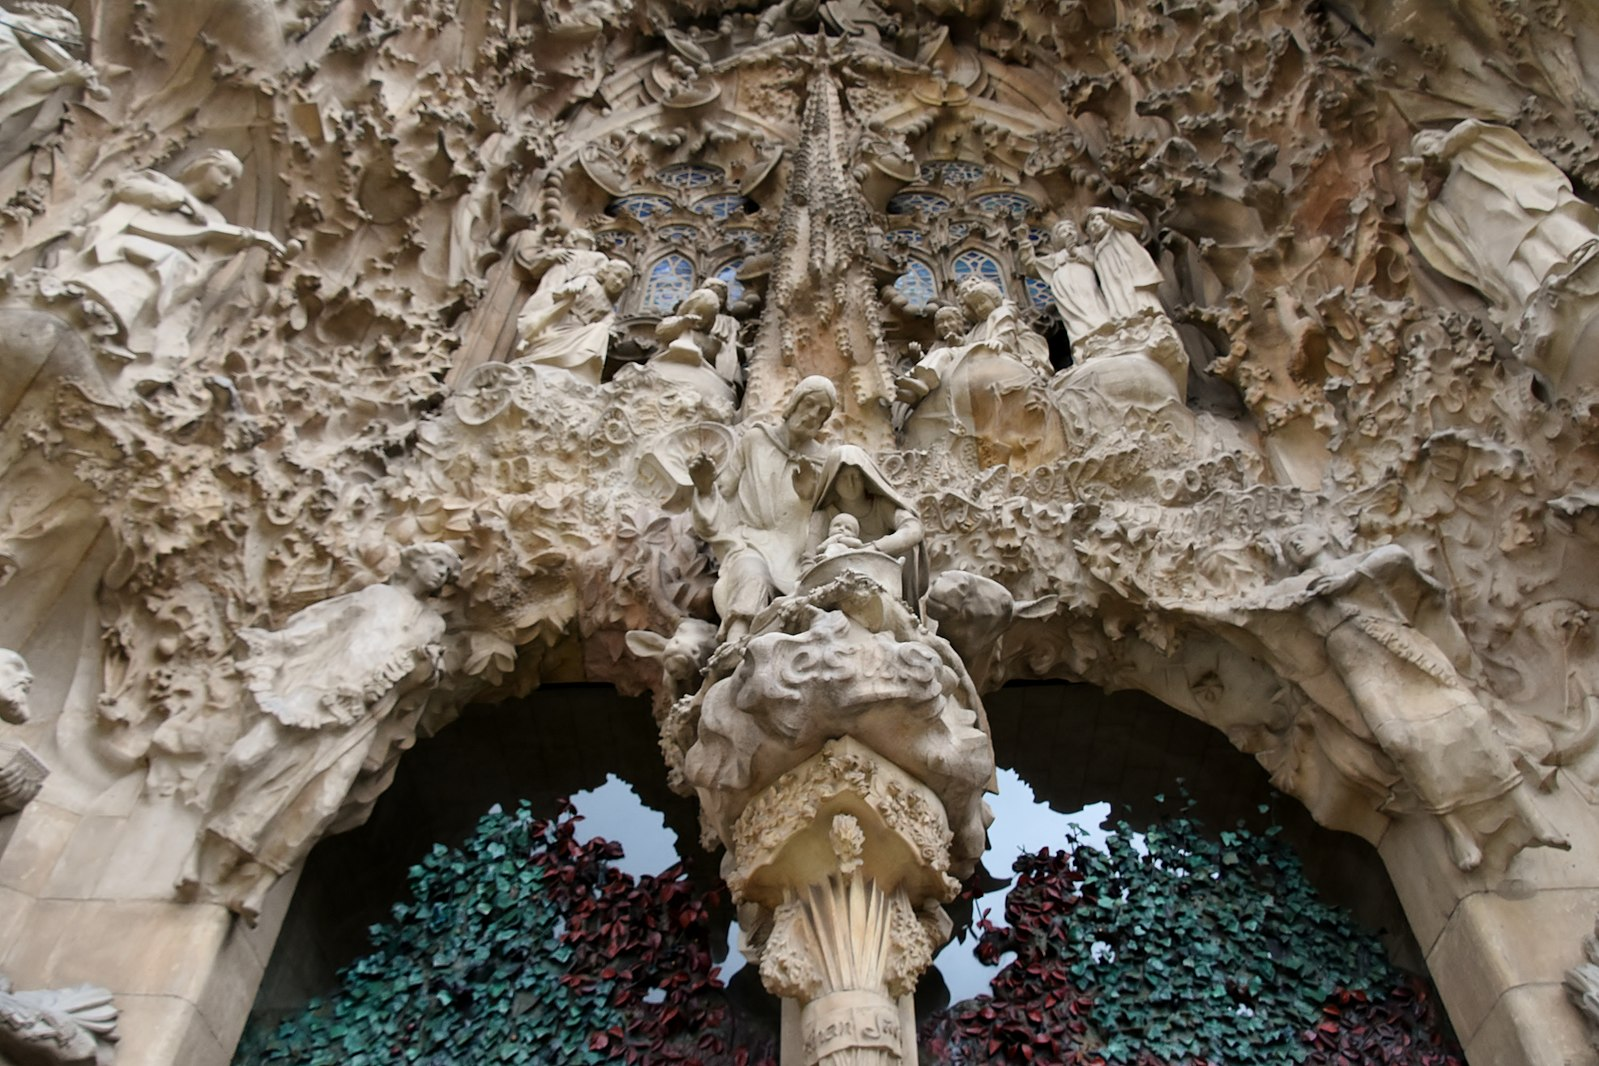
\includegraphics[height=4.75cm]{figures/sagrada_facade.jpg} }}
    \subfloat{{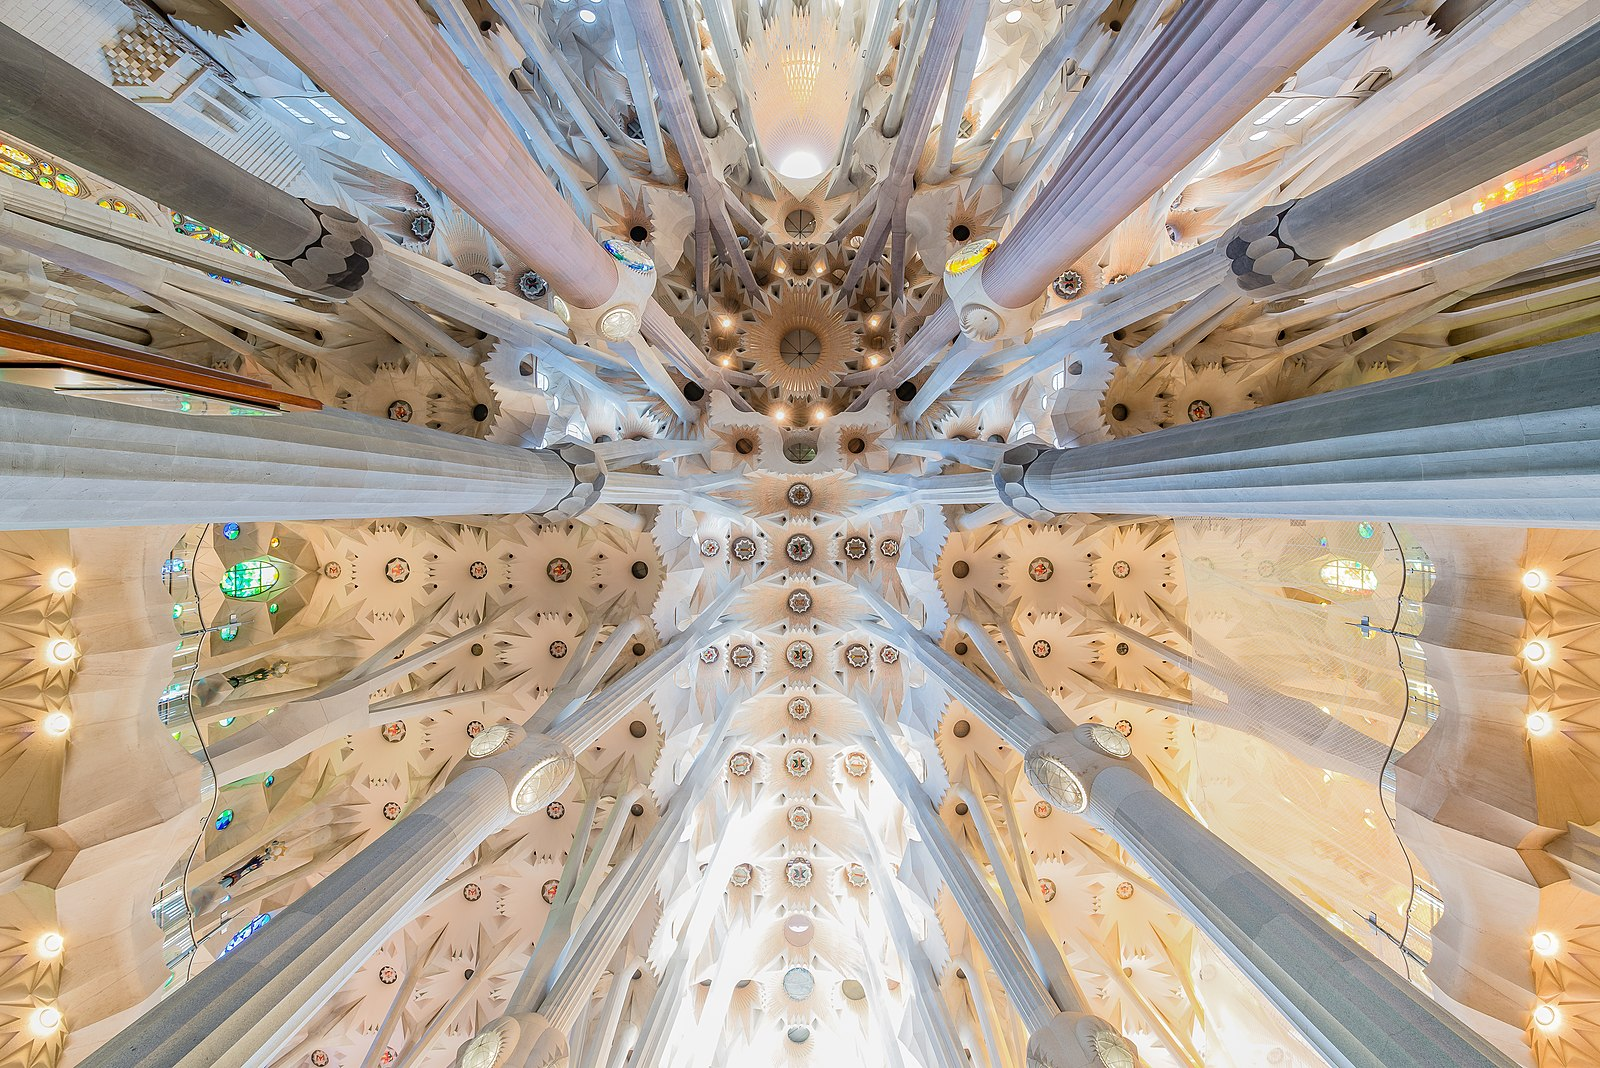
\includegraphics[height=4.75cm]{figures/sagrada_interior.jpg} }}
    \caption{Exterior and interior views of the Gothic Revival/Art Nouveau/Modernista style Catholic church \textit{Sagrada Familia} (en.: "Holy Family") in Barcelona, Spain, designed by Antoni Gaudí from 1883 until his death in 1926. Left: Details of the ornament-laden archway above the main gate of the nativity facade. Right: Wide-angle view of the arboreal load-bearing pillars in the nave. \newline Image sources (left to right): \cite{mortel_sagrada_2016}, \cite{wikimedia_commons_user_t_meltzer_sagrada_2014}.}
    \label{fig:sagrada}
\end{figure}

\begin{figure}
    \centering
    \subfloat{{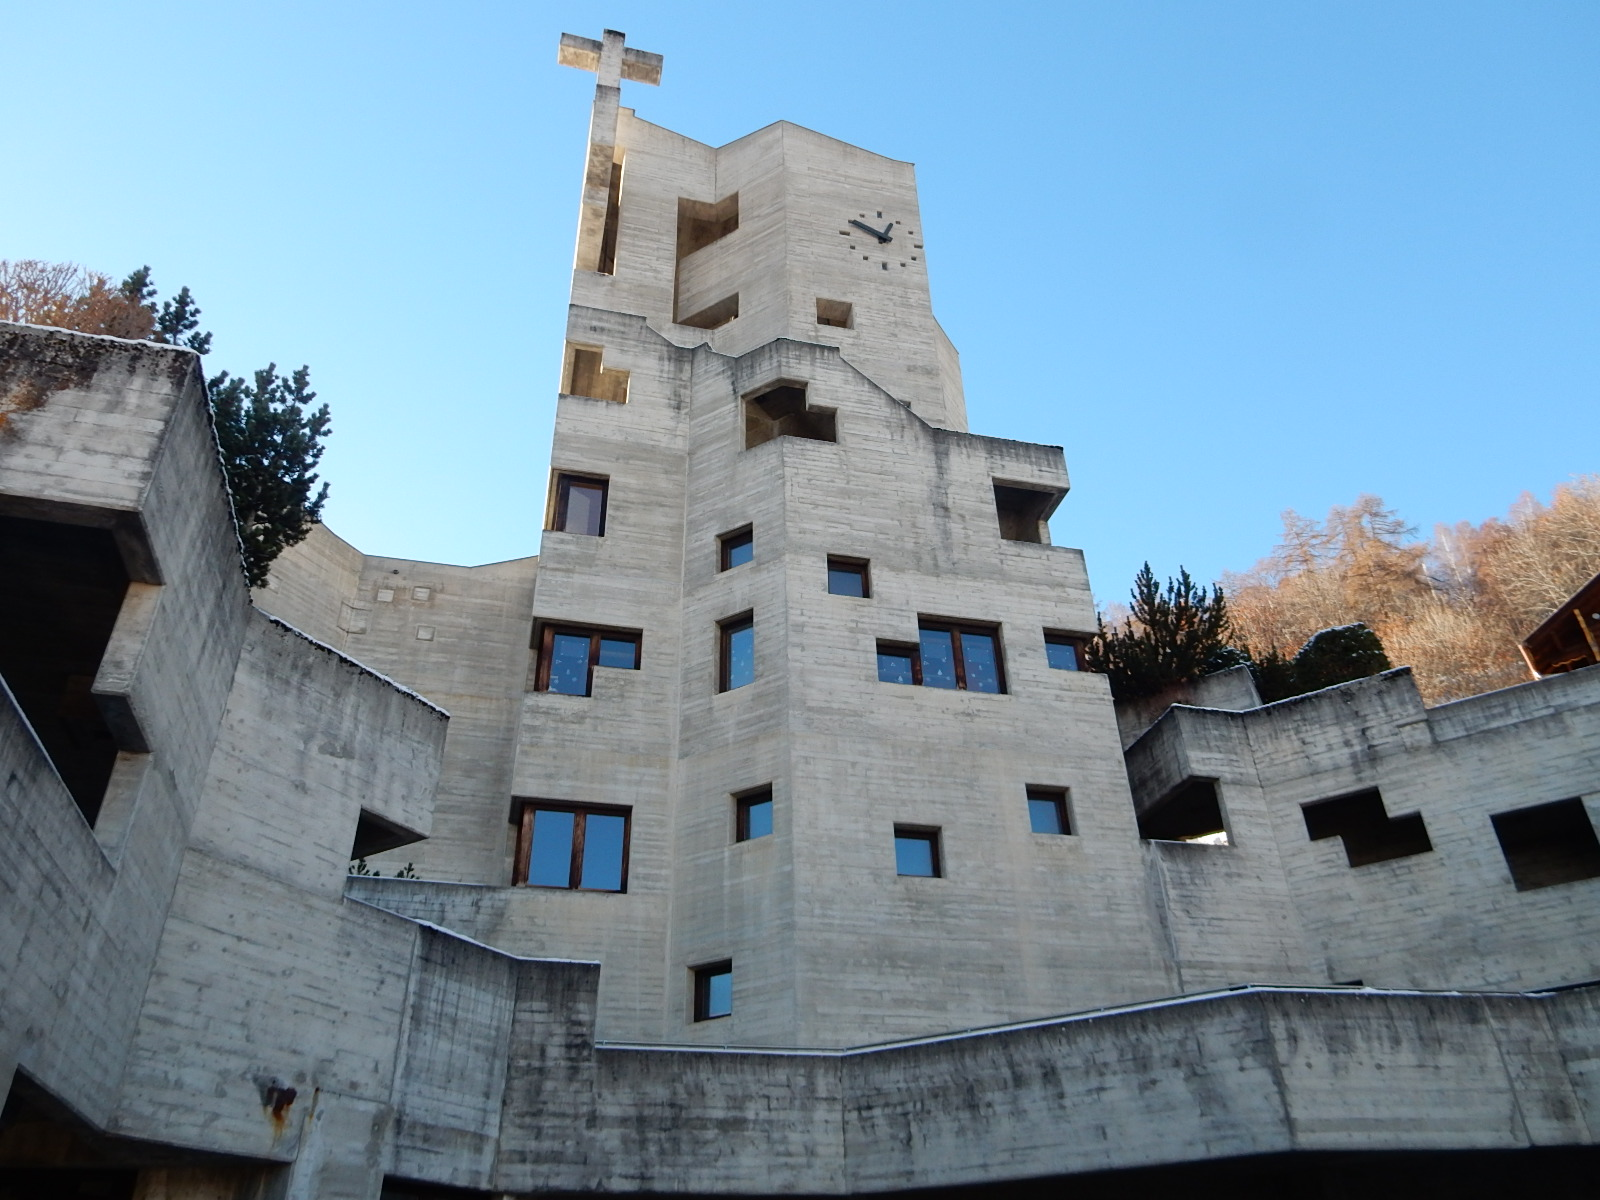
\includegraphics[height=4.5cm]{figures/hérémence_1.jpg} }}
    \subfloat{{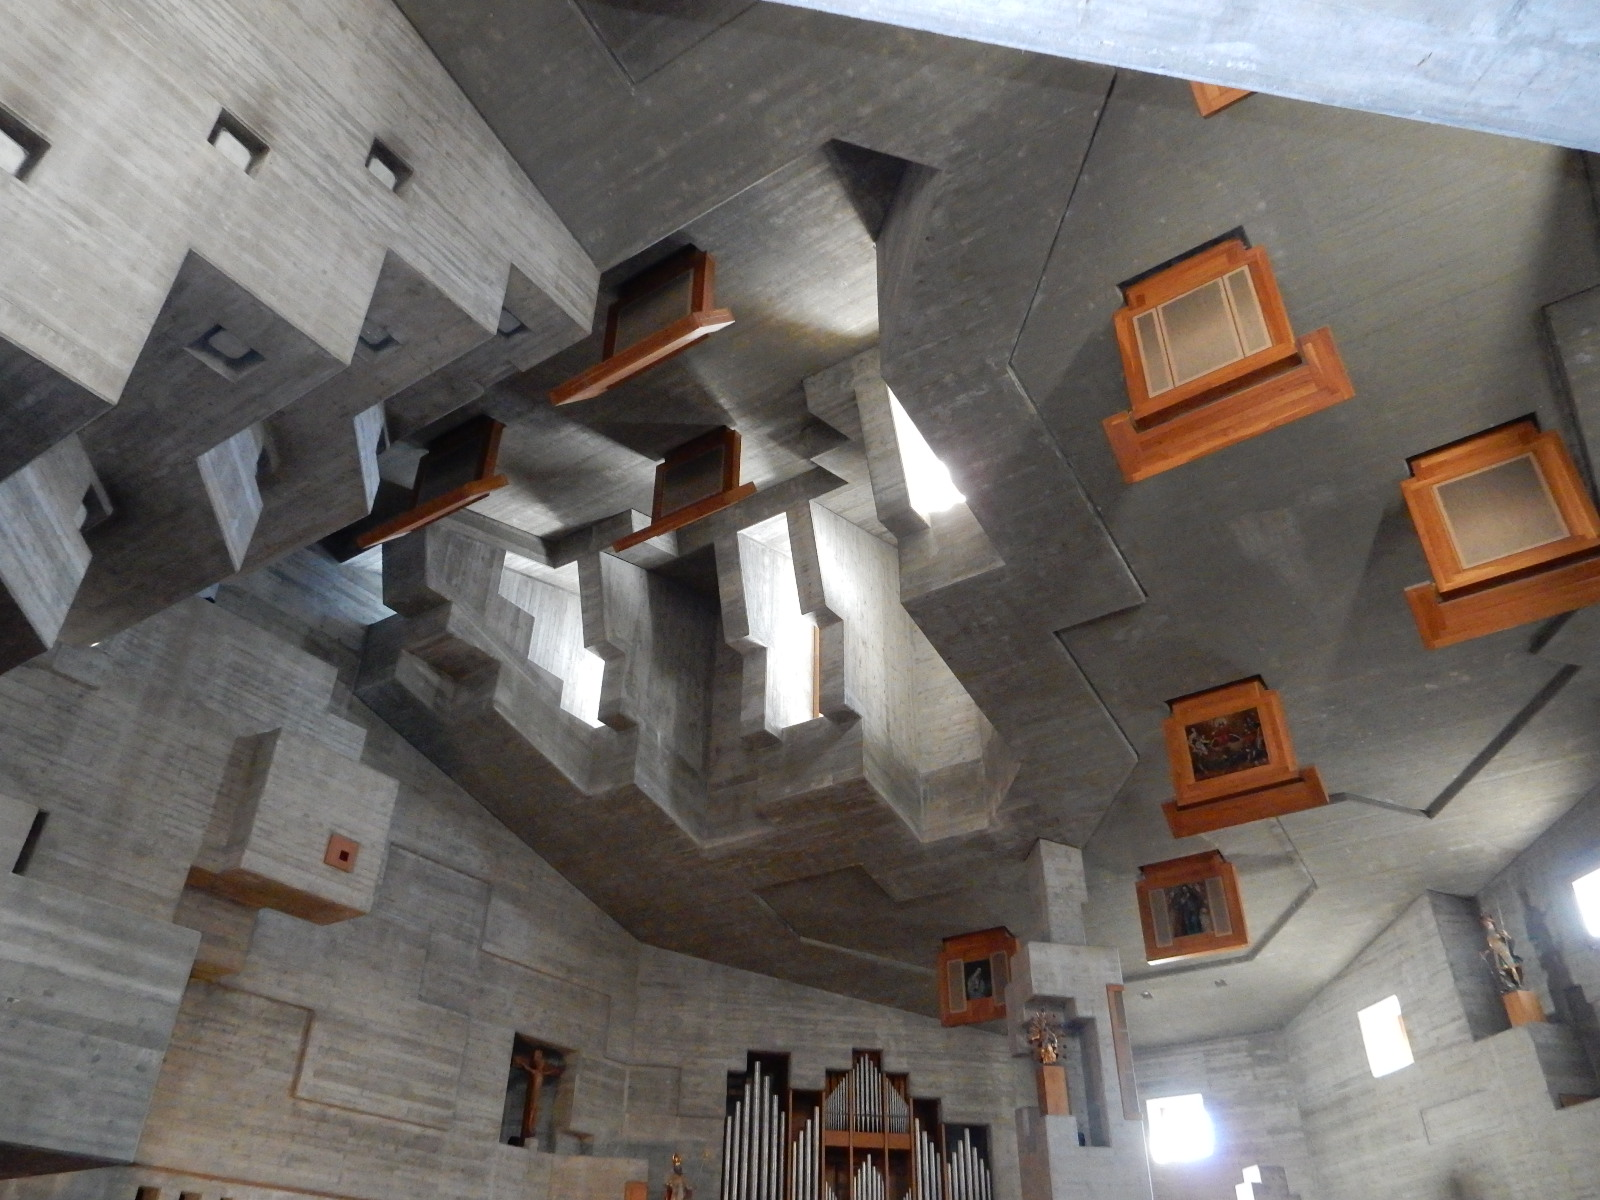
\includegraphics[height=4.5cm]{figures/hérémence_2.jpg} }}
    \caption{Brutalist-style catholic church "St. Nicolas" in the Swiss mountain village of Hérémence, designed by Walter Maria Förderer in 1967. Image sources from left to right: Outside view \cite{bissegger_eglise_2018-1} and inside view \cite{bissegger_eglise_2018}.}
    \label{fig:kunstformen}
\end{figure}

\clearpage
\printbibliography

\end{document}